\chapter{驾驶人行为特性对交通流影响}
\section{研究框架}
为了研究驾驶人行为特性对交通流的影响,由于交通流的复杂性。同时由于道路上的驾驶人个体,很难对其进行逐个的观测与调查,本文使用微观模拟的方法对驾驶人行为特性对交通流影响进行研究。
\subsection{模拟软件sumo简介}

根据Krajzewicz等(2006)\cite{Krajzewicz2006}
2000年起,德国航空中心(DLR)的交通研究所(IVF)开始开发微观交通模拟软件。并以开源的形式发布了整个软件包SUMO,作为交通研究中算法和模型的一般测试平台。SUMO为“Simulation of Urban MObility”的缩写,SUMO已被应用于模拟Magdeburg和Cologne,其研究主要关于交通管理和交通预测。

根据Krajzewicz等(2005)\cite{Krajzewicz2005},SUMO的默认值使用了Krauß跟驰模型,Krauß(1998)\cite{Krauss1998}提出了一个微观的空间连续跟驰模型,其主要基于安全速度假设,驾驶人为了对前车减速保有一定的安全余量,选择一定的距离和安全速度。模型假设驾驶人的反应时间tau为1s。并且SUMO可以很好的重现密度流量关系图。

\begin{figure}[!htb]
\begin{center}
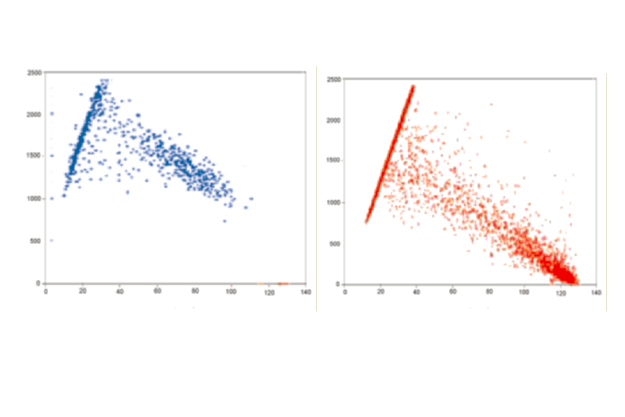
\includegraphics[width=\linewidth]{sumo}
\end{center}
\caption{sumo模拟密度-流量例图(摘自Krajzewicz等(2005)\cite{Krajzewicz2005})}
\label{sumo}
\end{figure}

Krauß模型给出如下:

\begin{equation}
v_{safe}=v_l(t)+\frac{g(t)-v_l(t)\tau}{\frac{\bar{v}}{b(\bar{v})}+\tau}
\end{equation}

其中:
\begin{displaymath}
{\begin{aligned}
v_l(t)&-t\text{时刻前车速度}\\
g(t)&-t\text{时刻与前车的空间间隔}\\
\tau&-\text{驾驶人的反应时间}\\
b&-t\text{减速函数}\\
\end{aligned}}
\end{displaymath}

为了保证车辆不超过其物理加速能力和最大速度,计算$v_{des}(t)$
\begin{equation}
v_{des}(t)=min[v_{safe},v(t)+a,v_{max}]
\end{equation}

最后从期望速度中减去随机项,使得模型变为随机
\begin{equation}
v_{t}(t)=max[0,rand[v_{des}(t)-\epsilon a,v_{des}(t)]]
\end{equation}



有效性

Ossen(2008)\cite{Ossen2008}研究表明,通过Gipps模型构造的人造轨迹数据对Tampère进行参数标定,结果表明即使模型不同,只要有足够的观测,仍可以对驾驶人的跟驰行为得出相似的理解。由于不存在完美的跟驰模型,但是人可以从实际观测数据对驾驶人行为作相互合理推断,同时相似结构的模型均可以揭示出驾驶人的行为特征。
因此,从前一章根据IDM模型得出的驾驶人差异性的结论仍可以认为对其他模型是成立的。

% Based on these results it seems justified to conclude that the true car-following behavior of the 
% observed follower can be identified by calibrating an “imperfect” model. 



Kerner\cite{S.Kerner2009}认为,传统的基于基本图的交通流理论不能解释,高速公路交通流的实际观测到的拥堵现象,提出了三相交通流理论。Kerner认为由于传统跟驰模型不能重现实际观测中的散落的密度-流量基本图,这一观点被Helbing认为是错误的,其评论Krauß模型认为由于Krauß模型,不能构成其认为的不连续超车概率因此不能解释F-S和S-J的相位变化。

Schönhof和Helbing\cite{Schoenhof2009}指出传统跟驰模型不能重现实际观测中的散落的密度-流量基本图,是由于未考虑驾驶人驾驶行为的差异性,传统模型的混合驾驶人模拟被证明可以重现实际观测中的散落的密度-流量基本图。


% IDM implementation

\subsection{模拟场景}


如图中,本文模拟场景设置为600m直线路段,单向3车道,为了增加扰动在路段末端设为2车道.共设置6个线圈检测器,分别在150m处和450m处。

\begin{figure}[!htb]
\begin{center}
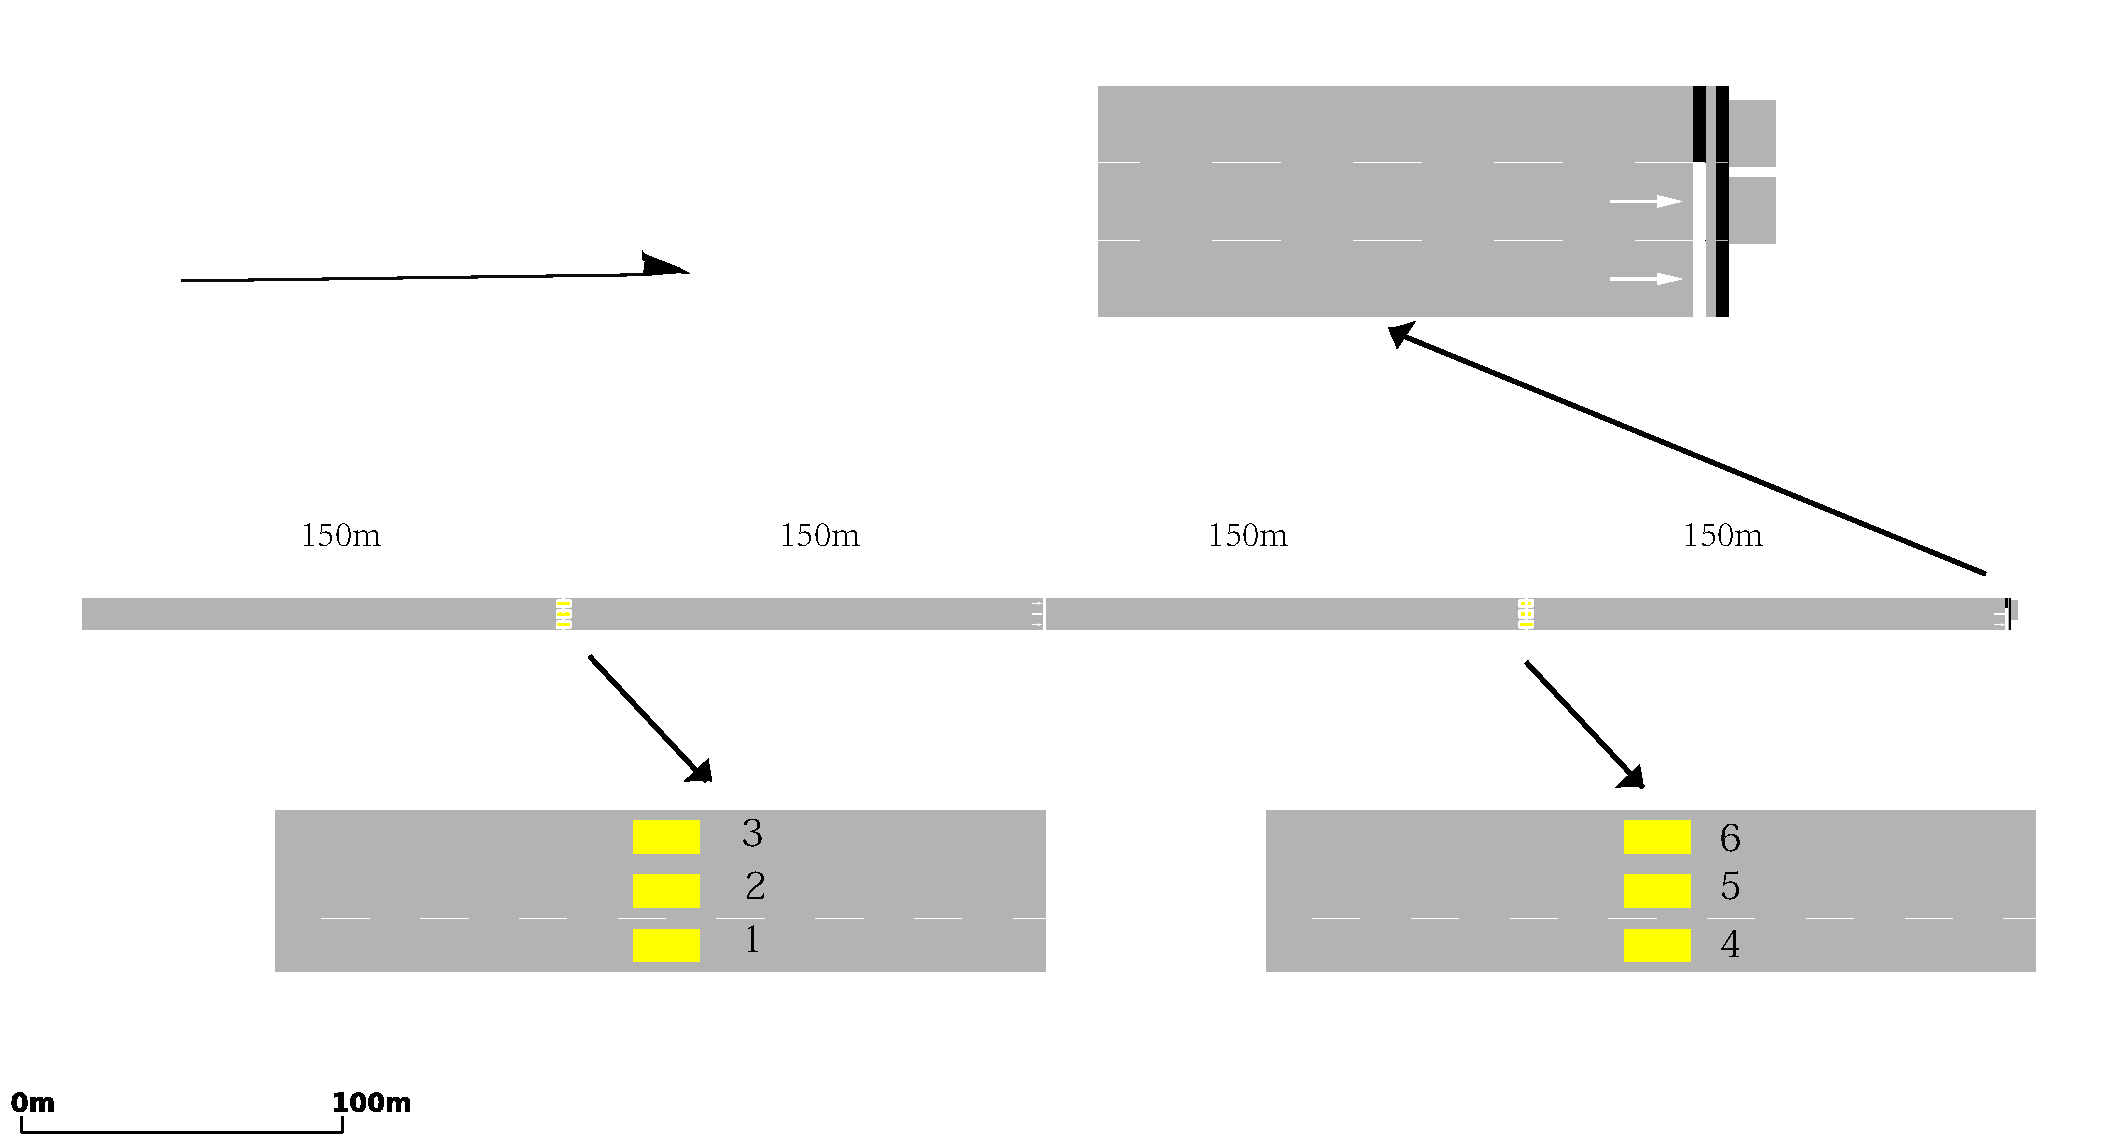
\includegraphics[width=\linewidth]{scene}
\end{center}
\caption{模拟场景图}
\label{scene}
\end{figure}

输入的交通流量,设置0-1200s,流率为600,1200-2400s,流率为1800,2400-4800s,流率为600,如\autoref{input-demand}

\begin{figure}[!htb]
\begin{center}
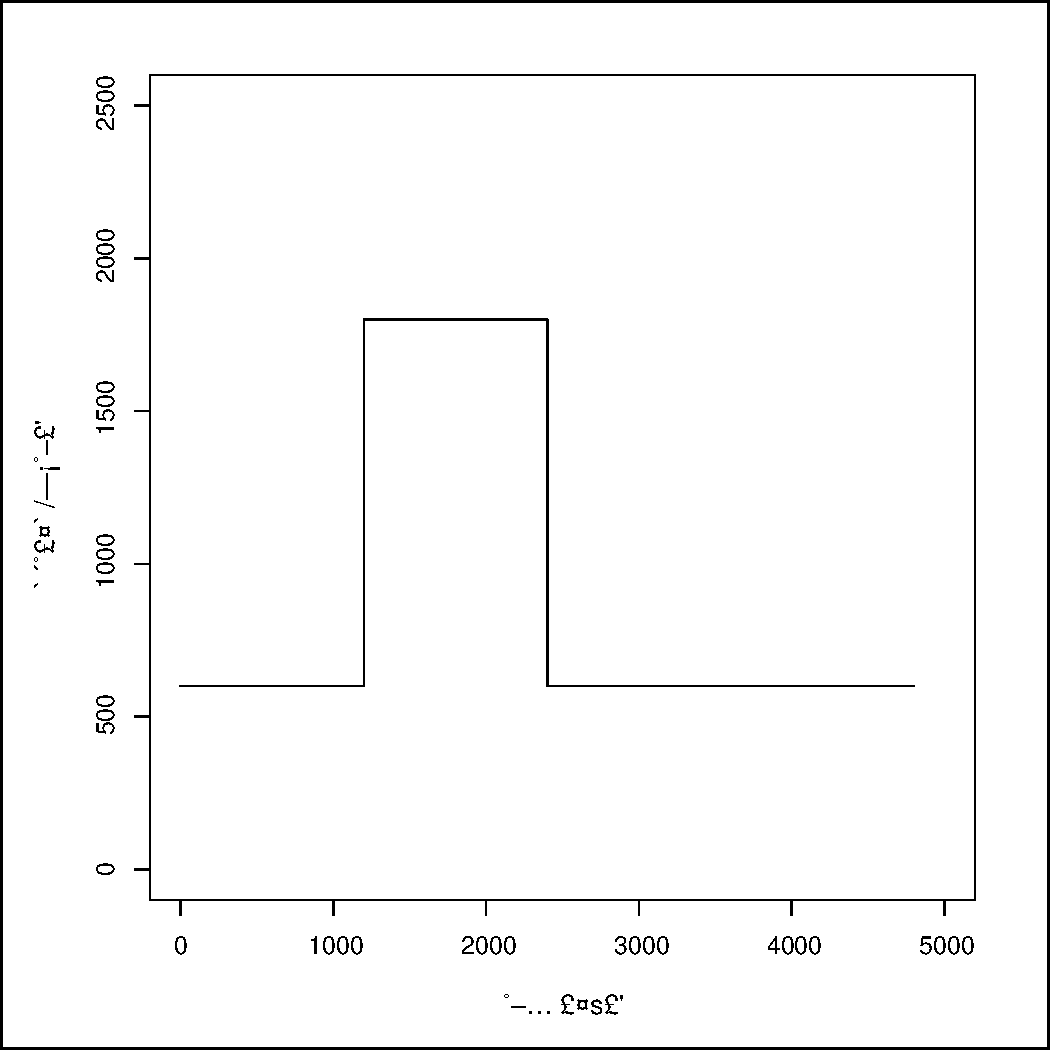
\includegraphics[width=0.3\linewidth]{input-demand}
\end{center}
\caption{交通需求随时间变化图}
\label{input-demand}
\end{figure}

为了研究驾驶人行为特性对交通流的影响,结合第四章所得结论。主要考察三种效应的影响,一为驾驶人期望车速对交通流的影响,二是驾驶人最大减速度对交通流的影响,三为两者混合效应的影响。

针对三种效应,对每一种效应分别选择两种车型,以全部A类型驾驶人,1:3,1:1和3:1的比例混合和全部B类型驾驶人分别进行模拟,也就是说B类型的驾驶人从0\%到25\%,50\%,75\%增加到100\%,由于在驾驶人混合中,车辆的出发顺序随机,在驾驶人混合中以不同随机种子数模拟10次。

\begin{table}[htb] 
  \begin{minipage}[b]{0.25\linewidth} 
  \centering
  \caption{期望速度的效应}
    \begin{tabular}{rrr}
    \addlinespace
    \toprule
    驾驶人类型    & A     & B \\
    \midrule
    最大加速度 & 0.62  & 0.62 \\
    最大减速度 & 2.33  & 2.33 \\
    期望速度  & 6.48  & 8.09 \\
    \bottomrule
    \end{tabular}%
  \label{speed-factor}%
  \end{minipage}% 
\hspace{0.08\linewidth}
  \begin{minipage}[b]{0.25\linewidth} 
  \centering
  \caption{最大减速度的效应}
    \begin{tabular}{rrr}
    \addlinespace
    \toprule
    驾驶人类型    & A     & B \\
    \midrule
    最大加速度 & 0.62  & 0.62 \\
    最大减速度 & 2.33  & 4.29 \\
    期望速度  & 8.09  & 8.09 \\
    \bottomrule
    \end{tabular}%
  \label{decel-factor}%
  \end{minipage}
\hspace{0.08\linewidth}
  \begin{minipage}[b]{0.25\linewidth} 
  \centering
  \caption{混合效应}
    \begin{tabular}{rrr}
    \addlinespace
    \toprule
    驾驶人类型    & A     & B \\
    \midrule
    最大加速度 & 0.62  & 0.62 \\
    最大减速度 & 2.33  & 4.29 \\
    期望速度  & 8.09  & 6.48 \\
    \bottomrule
    \end{tabular}%
  \label{combined-factor}%
  \end{minipage} 
\end{table}






\subsection{评价指标}
效率性,主要从基本图来看交通流效率性的影响
安全性,以TTC倒数的和来评价安全性


\section{对交通流效率性}

\subsection{期望速度影响因素}
根据\autoref{speed-factor}的驾驶人参数进行混合模拟,得到:

\begin{figure}[!htb]
\begin{center}
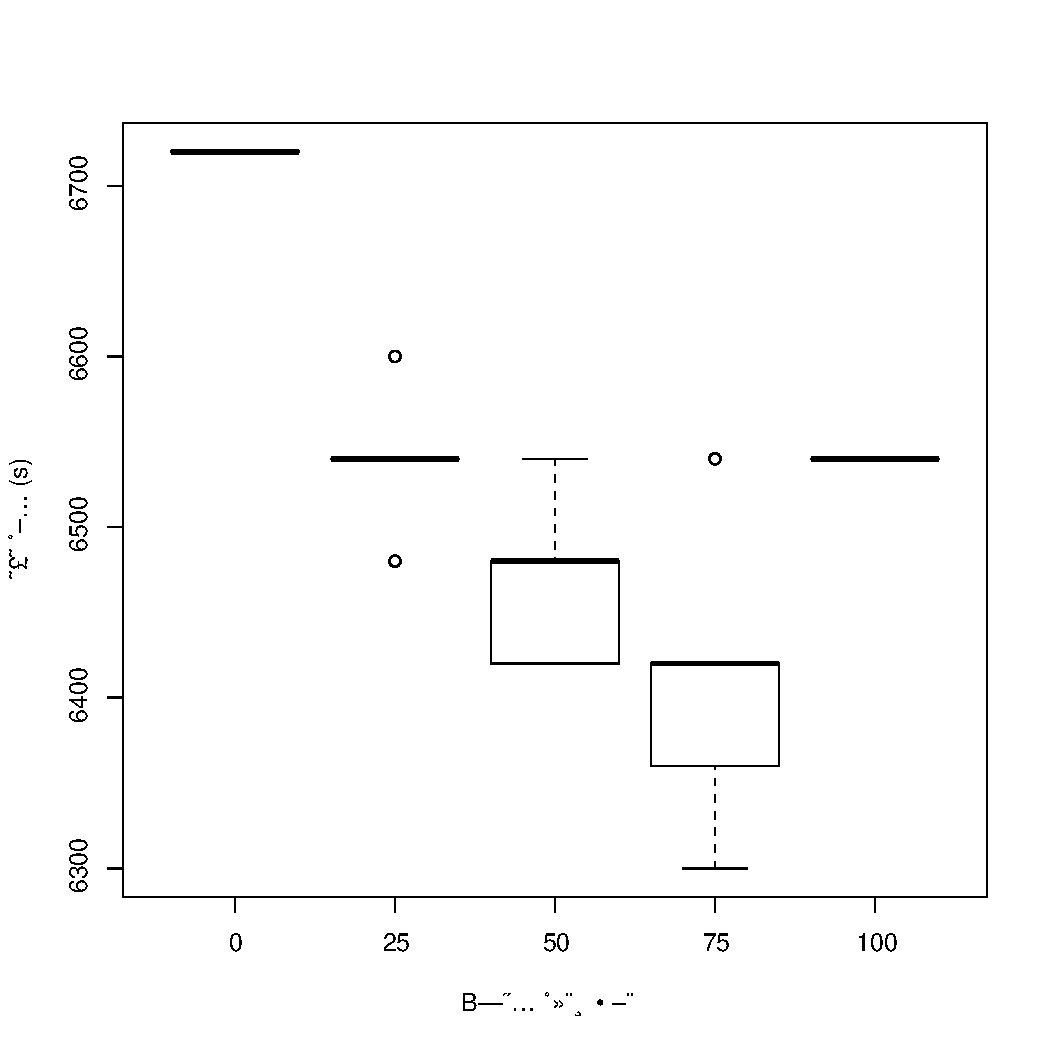
\includegraphics[width=0.5\linewidth]{factor1_box_ttime}
\caption{期望速度影响下模拟用时箱图}
\label{factor1_box_ttime}
\end{center}
\end{figure}

\autoref{factor1_box_ttime}给出了,期望速度影响下模拟总用时的变化,随着\autoref{speed-factor}中期望速度较大的B型驾驶人的增加,模拟所用时间呈现下降的趋势。对于单纯类型的驾驶人组合,期望速度由6.48m/s(23.3km/h)增加8.09m/s(30.6km/h),增加24.8\%,模拟用时从6720s下降到6540s,降低了3\%。

对速度-流量图形状的影响


\begin{figure}[!htb]%
\centering
\subfloat[][]{
\label{factor1_vq_per0}%
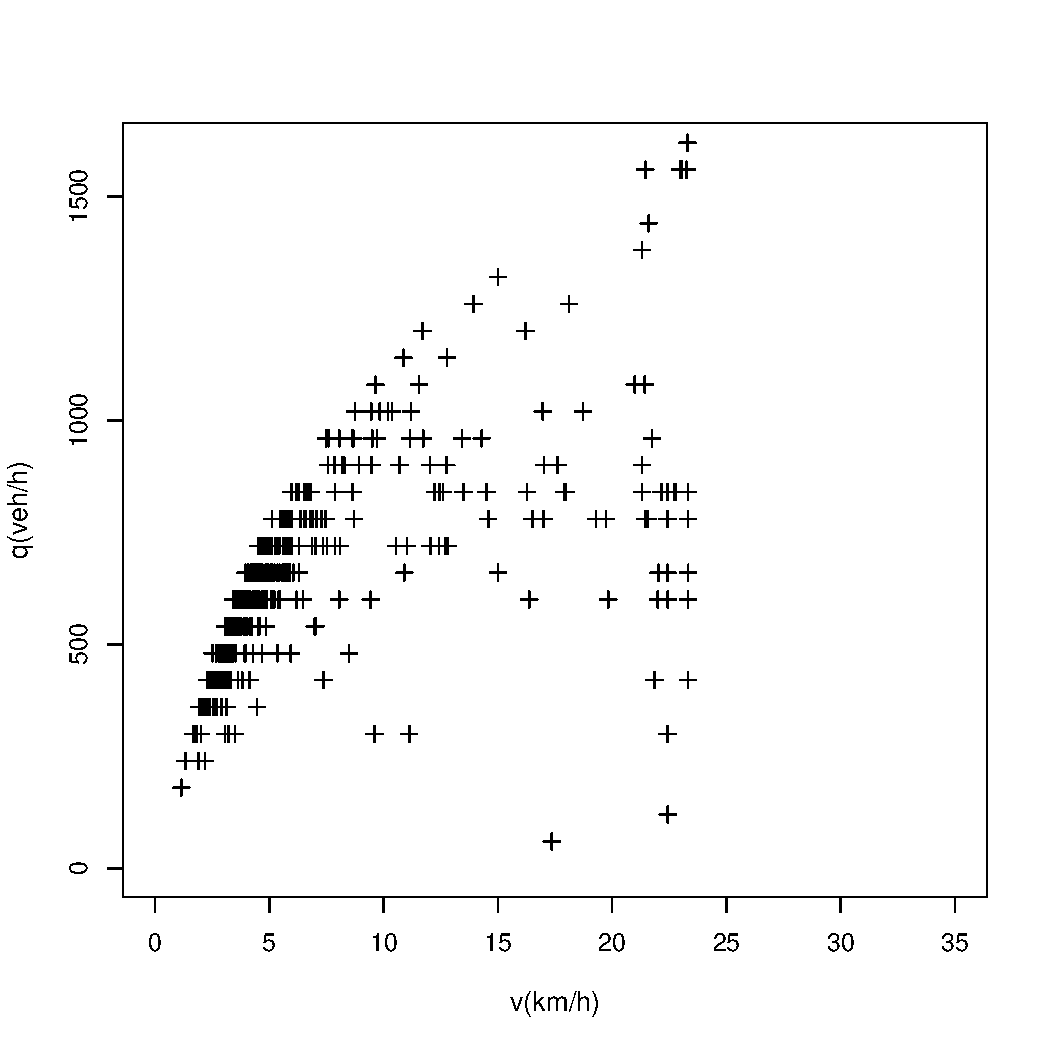
\includegraphics[width=0.33\linewidth]{factor1_vq_per0}
}%
\subfloat[][]{%
\label{factor1_vq_per25}%
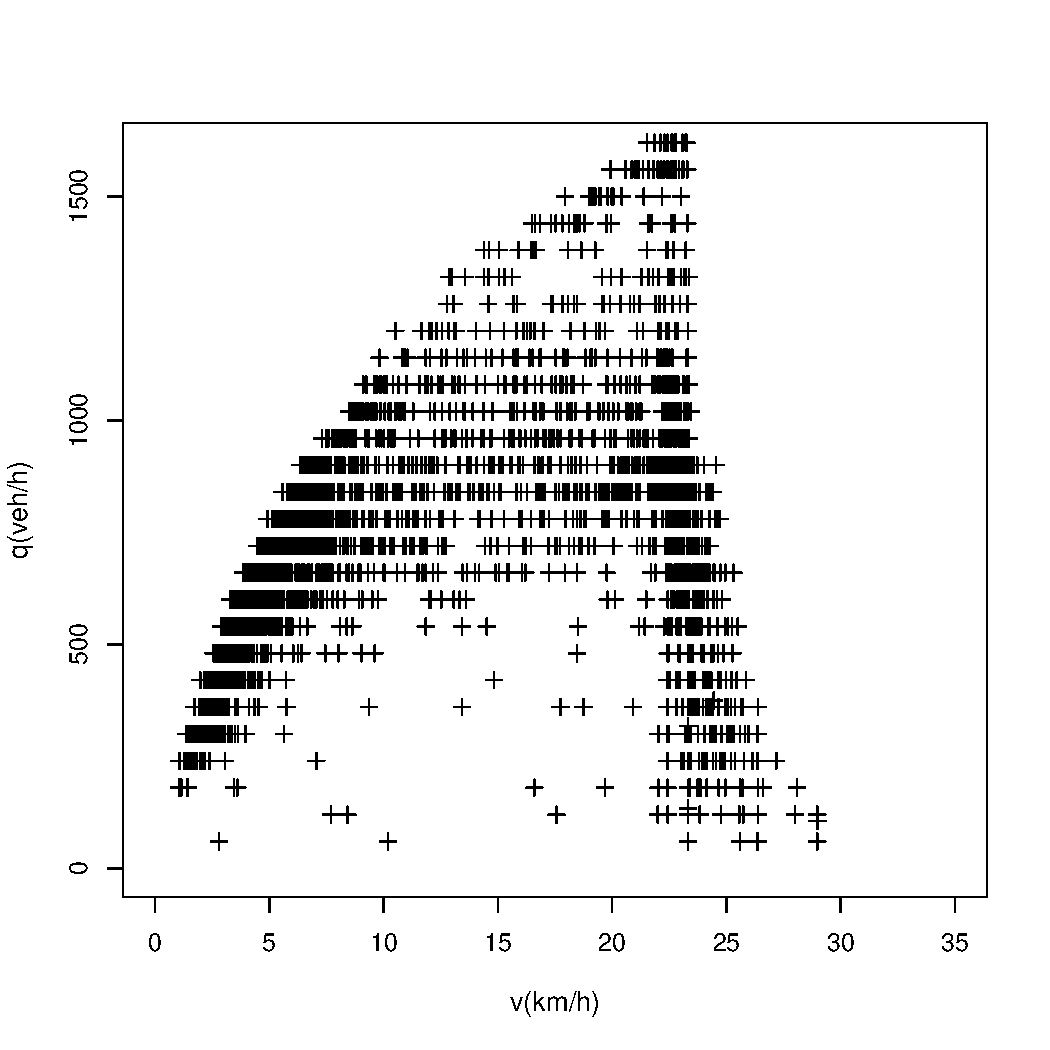
\includegraphics[width=0.33\linewidth]{factor1_vq_per25}}
\subfloat[][]{%
\label{factor1_vq_per50}%
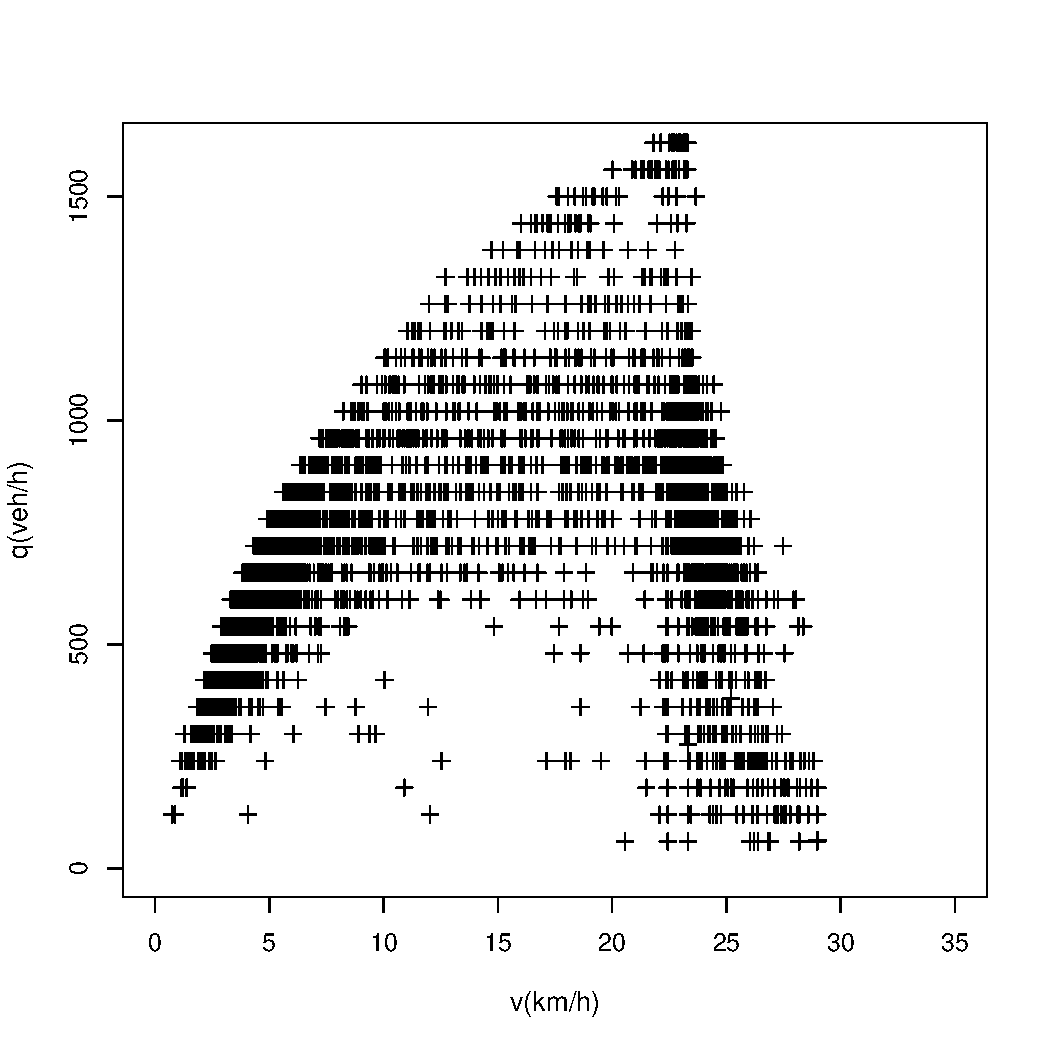
\includegraphics[width=0.33\linewidth]{factor1_vq_per50}}\\%
\subfloat[][]{%
\label{factor1_vq_per75}%
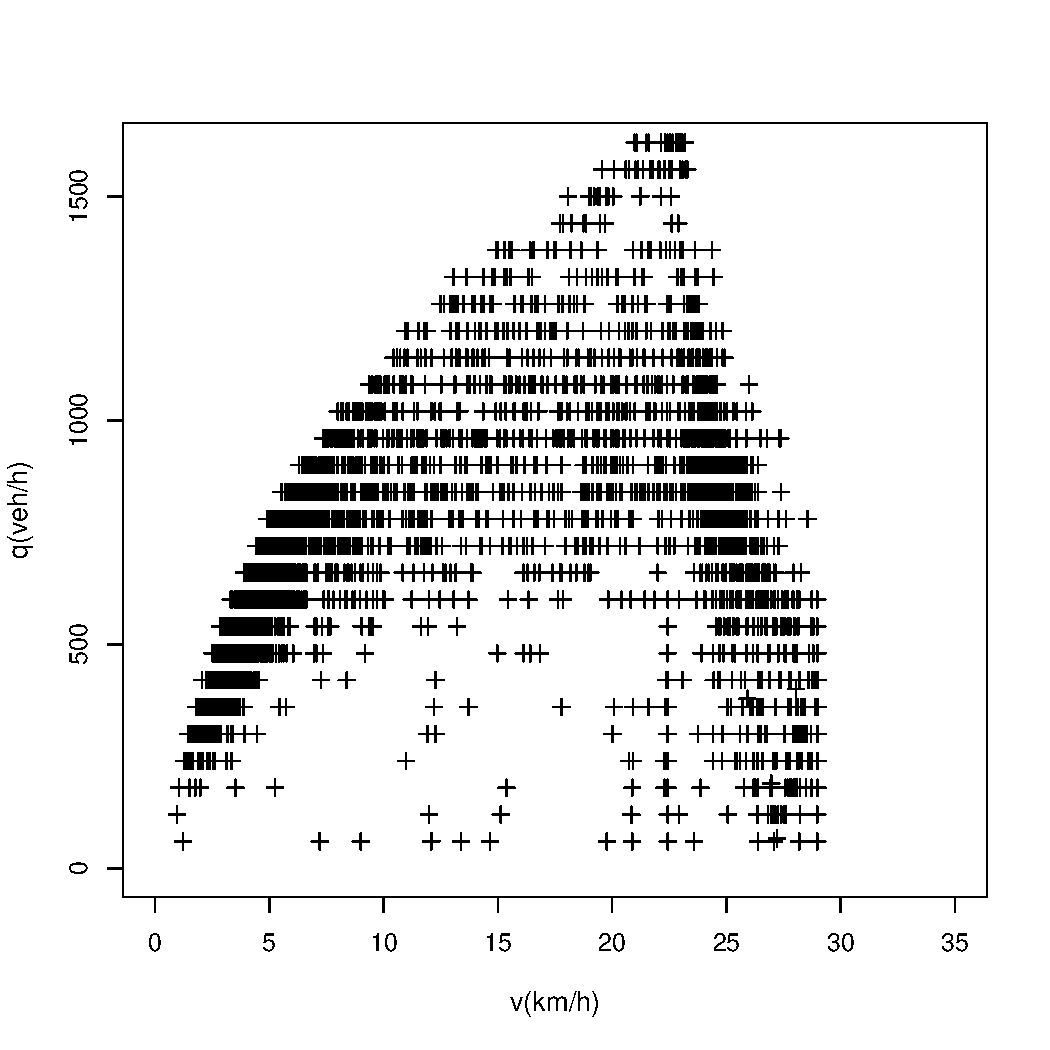
\includegraphics[width=0.33\linewidth]{factor1_vq_per75}}%
\subfloat[][]{%
\label{factor1_vq_per100}%
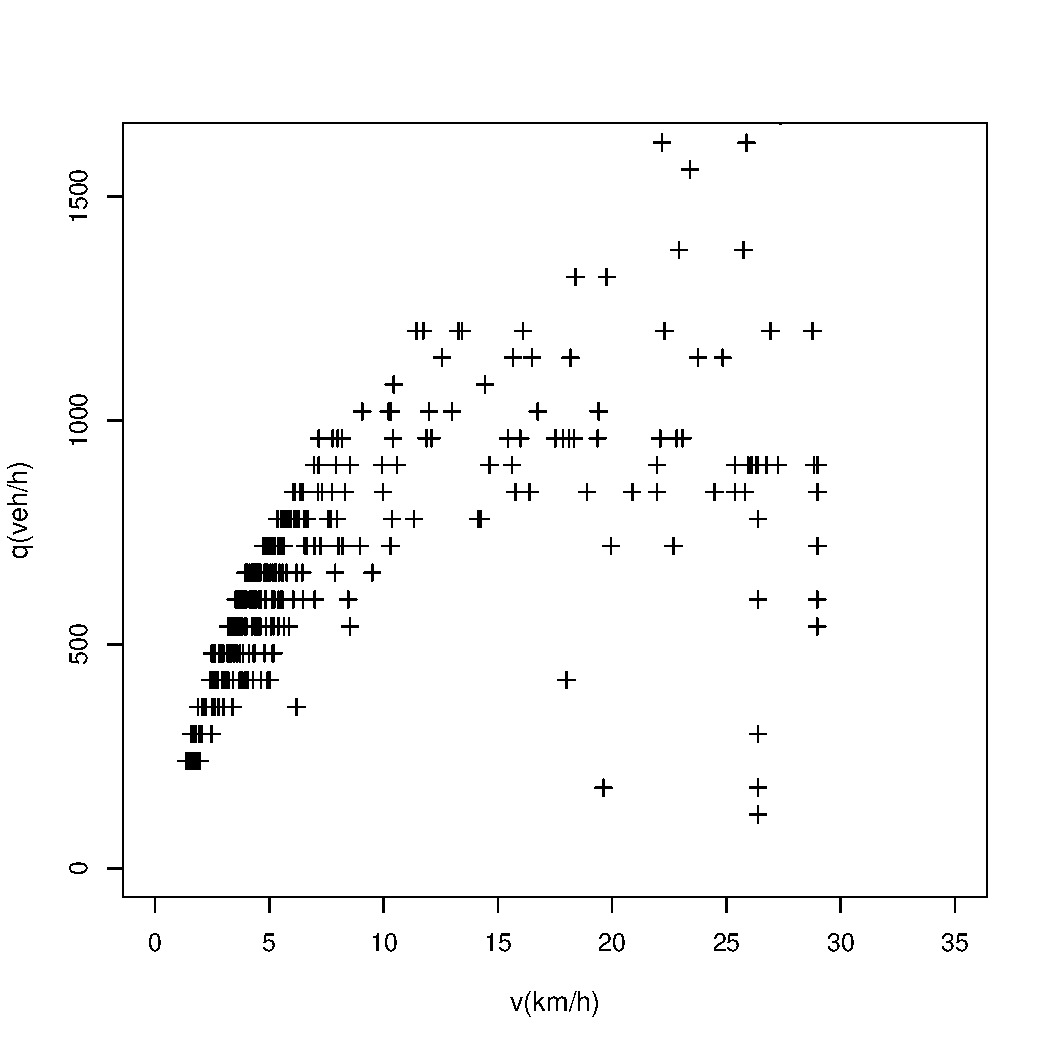
\includegraphics[width=0.33\linewidth]{factor1_vq_per100}}
\caption[A set of four sub-floats.]{期望速度影响下速度流量关系图
\subref{factor1_vq_per0}
\subref{factor1_vq_per25} 
\subref{factor1_vq_per50}
\subref{factor1_vq_per75}
\subref{factor1_vq_per100}分别表示\autoref{speed-factor}中的B型驾驶人的百分比分别为0\%,25\%,50\%,75\%,100\%}%
\label{factor1_vq}%
\end{figure}

由\autoref{factor1_vq}看出,期望速度主要对速度-流量关系图中的形状有影响,对最大通行能力和最大通行能力所对应的最佳车速基本没有影响,图中可以看出最大通行能力约为1600veh/h,最佳速度大约均在22km/h。期望速度对速度-流量关系图中的形状的影响主要体现在,最佳车速的右侧主要为自由流的阶段。由于两组的期望速度均超过了最佳车速,因此不能排除当期望速度低于最佳车速时可能会对最大通行能力产生影响。



\begin{figure}[!htb]%
\centering
\subfloat[][]{
\label{factor1_kq_per0}%
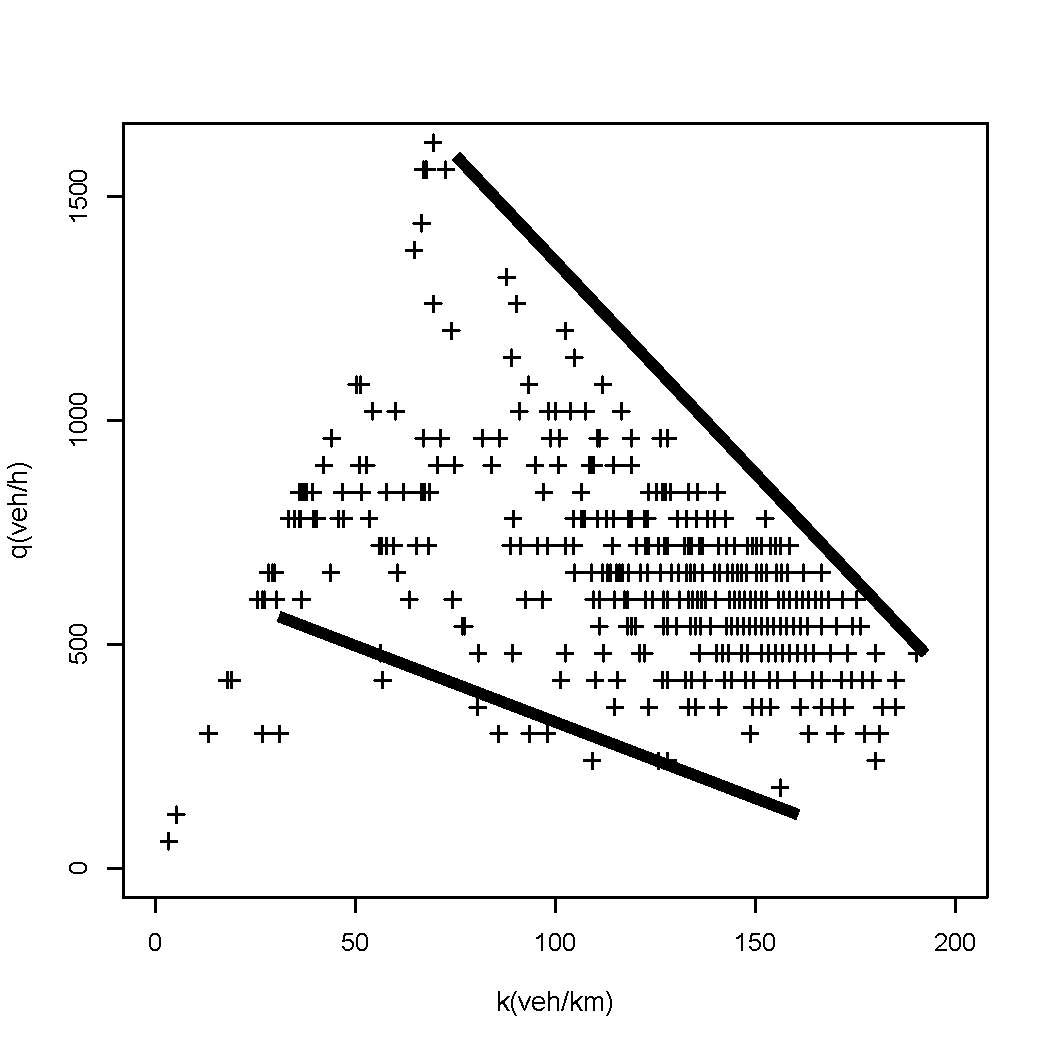
\includegraphics[width=0.33\linewidth]{factor1_kq_per0}
}%
\subfloat[][]{%
\label{factor1_kq_per25}%
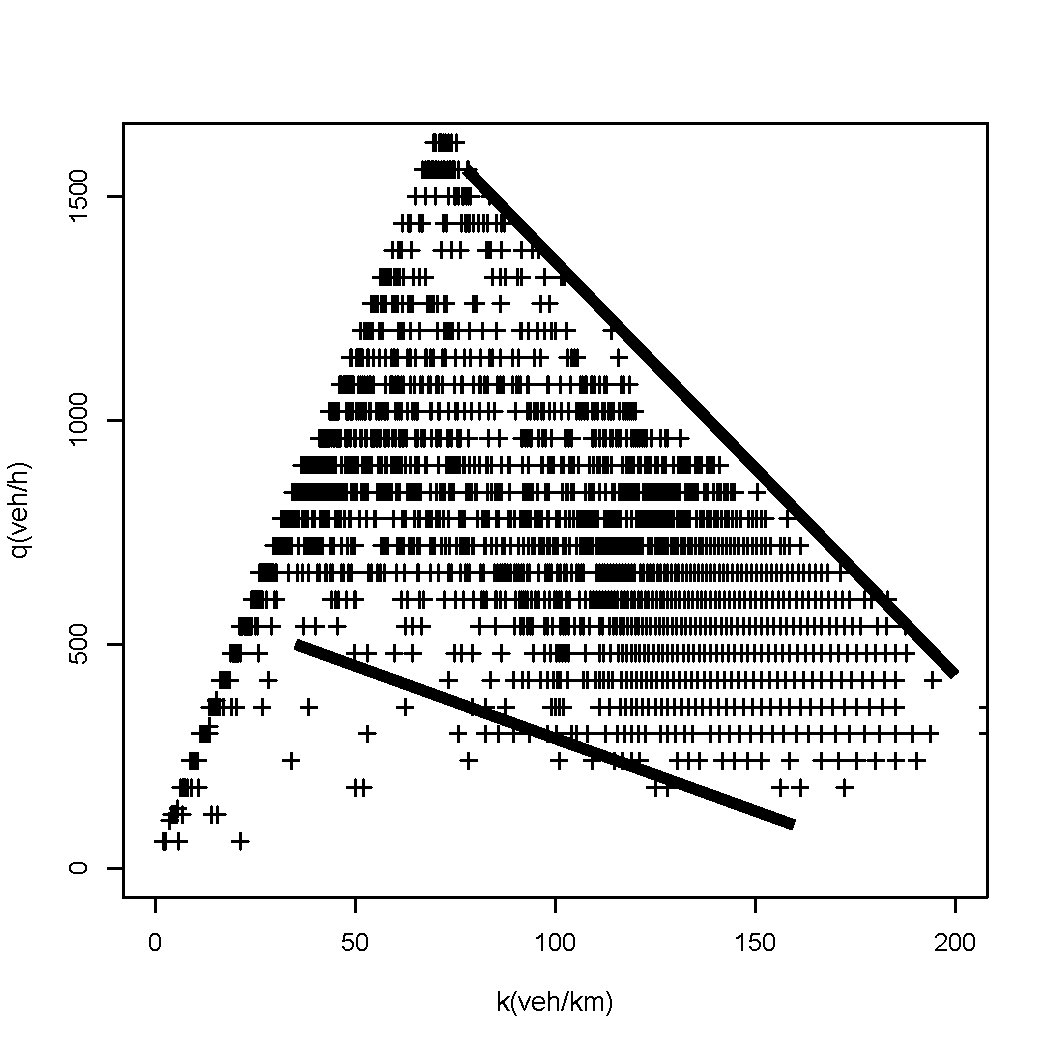
\includegraphics[width=0.33\linewidth]{factor1_kq_per25}}
\subfloat[][]{%
\label{factor1_kq_per50}%
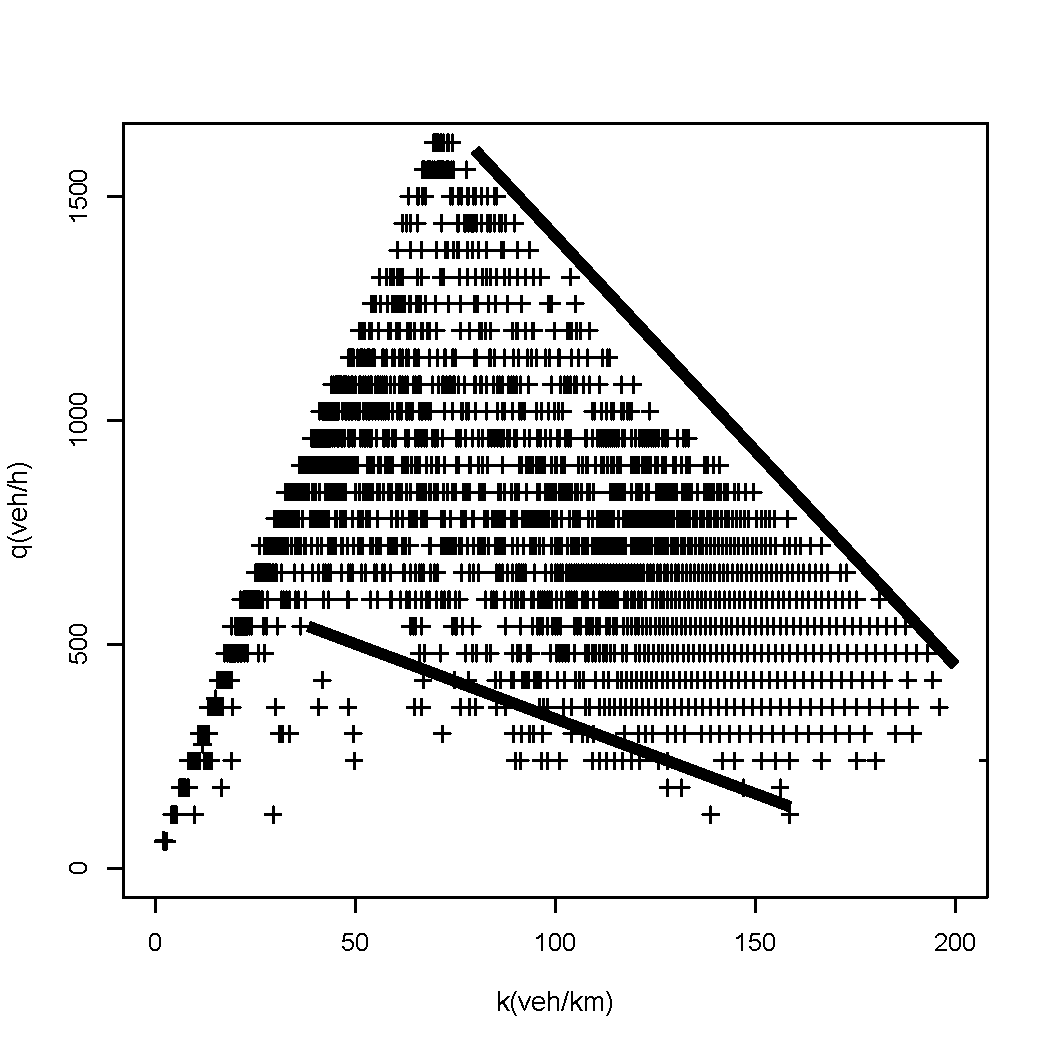
\includegraphics[width=0.33\linewidth]{factor1_kq_per50}}\\%
\subfloat[][]{%
\label{factor1_kq_per75}%
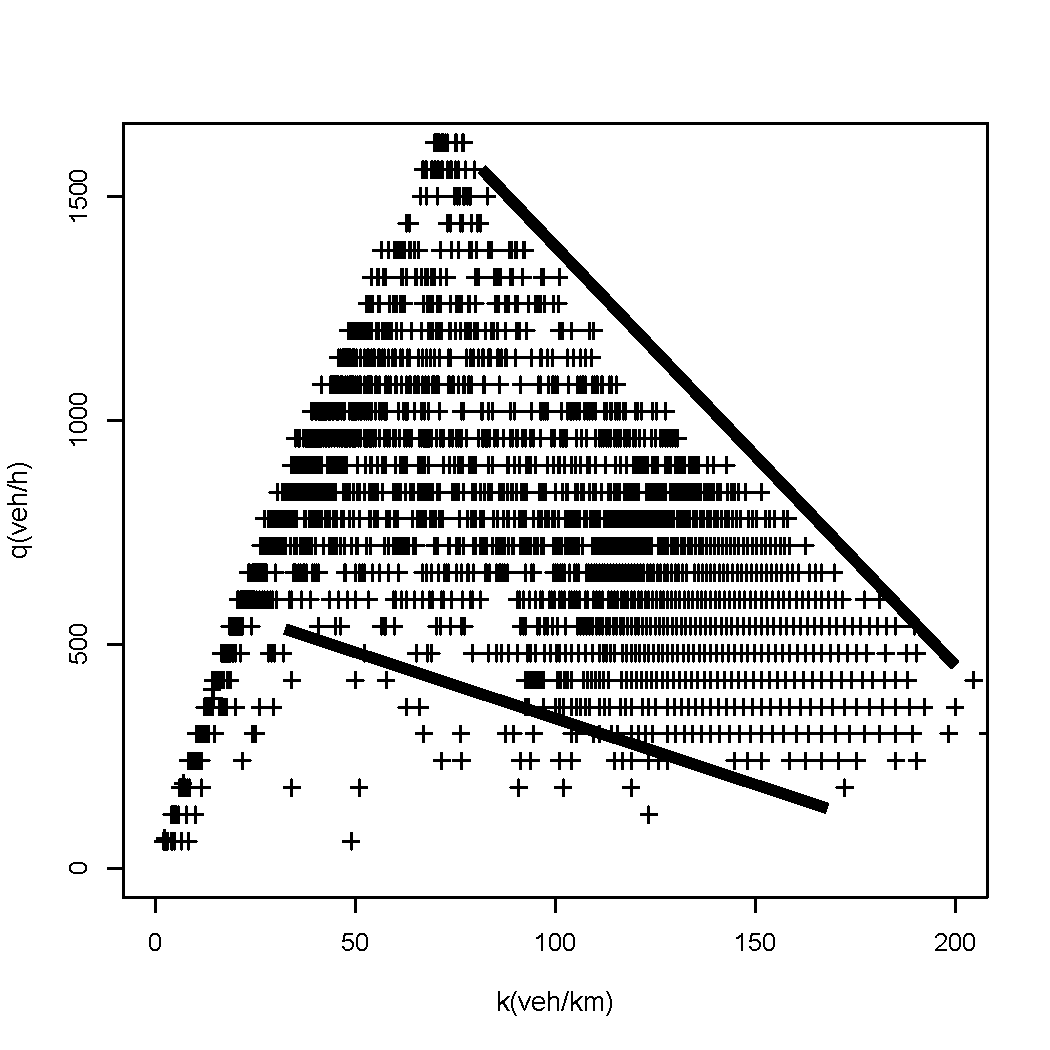
\includegraphics[width=0.33\linewidth]{factor1_kq_per75}}%
\subfloat[][]{%
\label{factor1_kq_per100}%
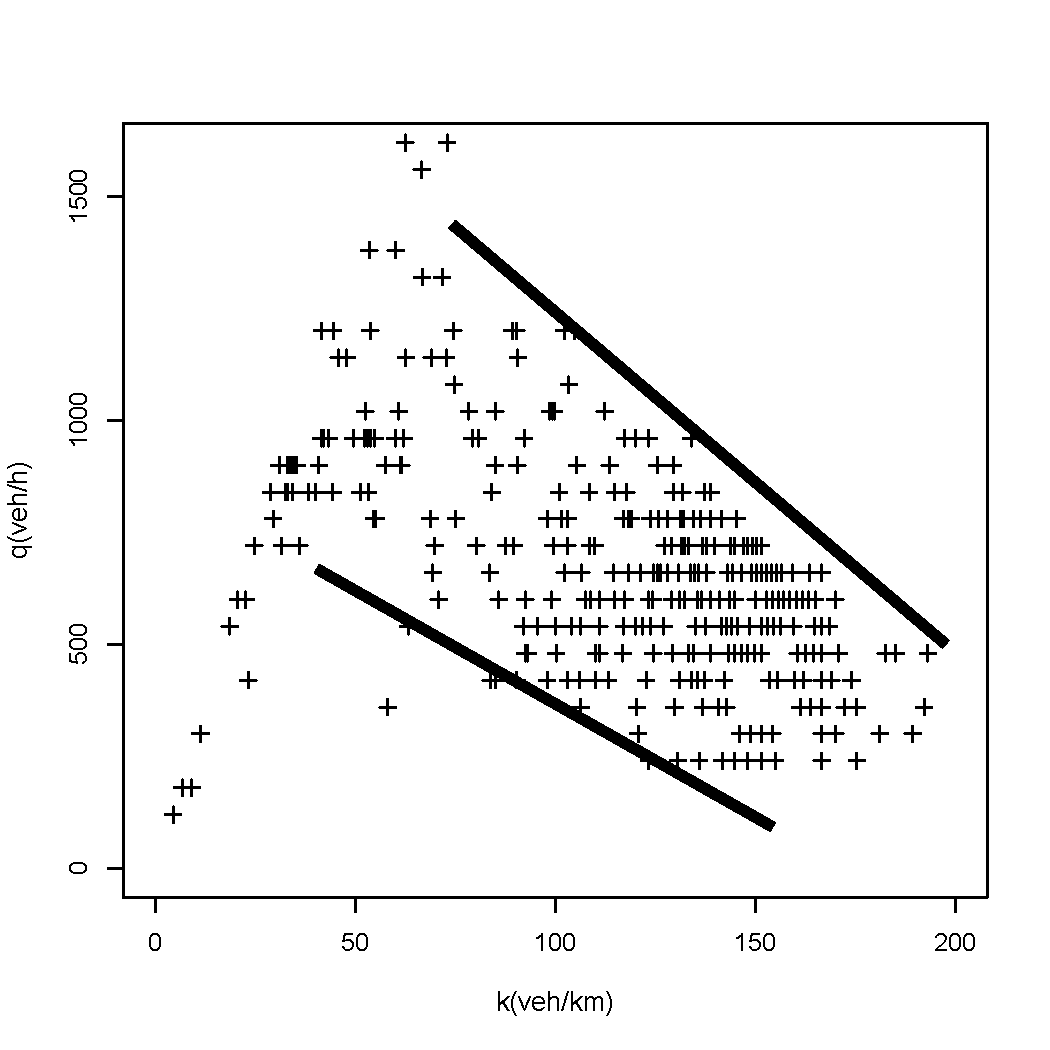
\includegraphics[width=0.33\linewidth]{factor1_kq_per100}}
\caption[A set of four sub-floats.]{期望速度影响下的密度流量关系图
\subref{factor1_kq_per0}
\subref{factor1_kq_per25} 
\subref{factor1_kq_per50}
\subref{factor1_kq_per75}
\subref{factor1_kq_per100}分别表示\autoref{speed-factor}中的B型驾驶人的百分比分别为0\%,25\%,50\%,75\%,100\%}%
\label{factor1_kq}%
\end{figure}

由\autoref{factor1_kq}看,期望速度对最佳密度基本没有影响。根据Kerner的三相交通流理论,道路介于最大和最小通行能力之间具有无数个通行能力,\autoref{factor1_kq}中e的最小通行能力稍大于其他的情况,这似乎表明最小通行能力受到最低期望车速的影响。由于低期望车速的驾驶人的存在,???根据三相交通流中Speed adaptation效用的作用,低速车辆的阻碍造成最低通行能力的下降是可以理解的。

\subsection{最大减速度影响因素}

\begin{figure}[!htb]
\begin{center}
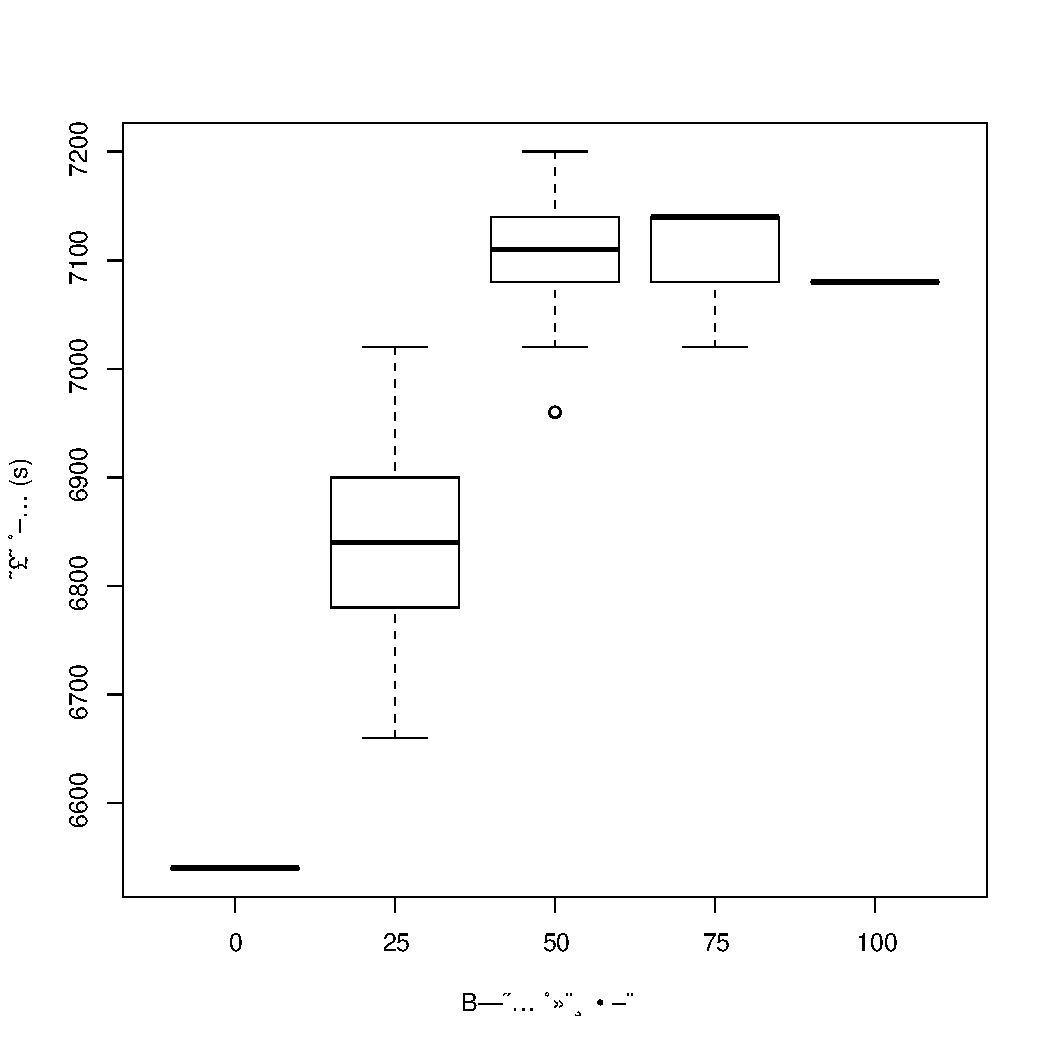
\includegraphics[width=0.5\linewidth]{factor2_box_ttime}
\caption{最大减速度影响下模拟用时箱图}
\label{factor2_box_ttime}
\end{center}
\end{figure}

\autoref{factor2_box_ttime}给出了,期望速度影响下模拟总用时的变化,随着\autoref{decel-factor}中最大减速度较大的B型驾驶人的增加,模拟所用时间呈现上升的趋势。对于单纯类型的驾驶人组合,最大减速度由2.33$m/s^2$增加4.29$m/s^2$,增加84\%,模拟用时从6540s增加到7080s,增加了8.3\%。

少量的B型驾驶人即可对总模拟用时造成较大影响。


\begin{figure}[!htb]%
\centering
\subfloat[][]{
\label{factor2_vq_per0}%
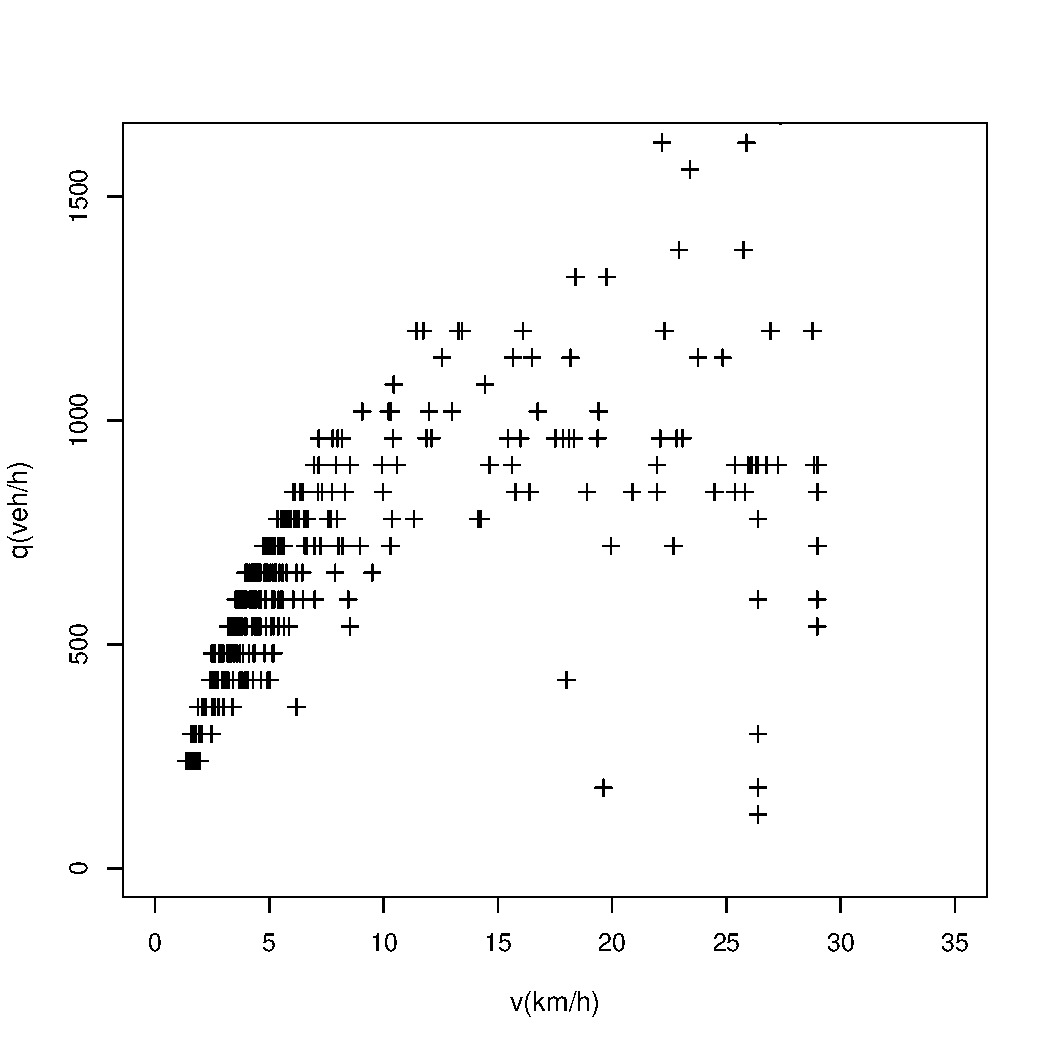
\includegraphics[width=0.33\linewidth]{factor2_vq_per0}
}%
\subfloat[][]{%
\label{factor2_vq_per25}%
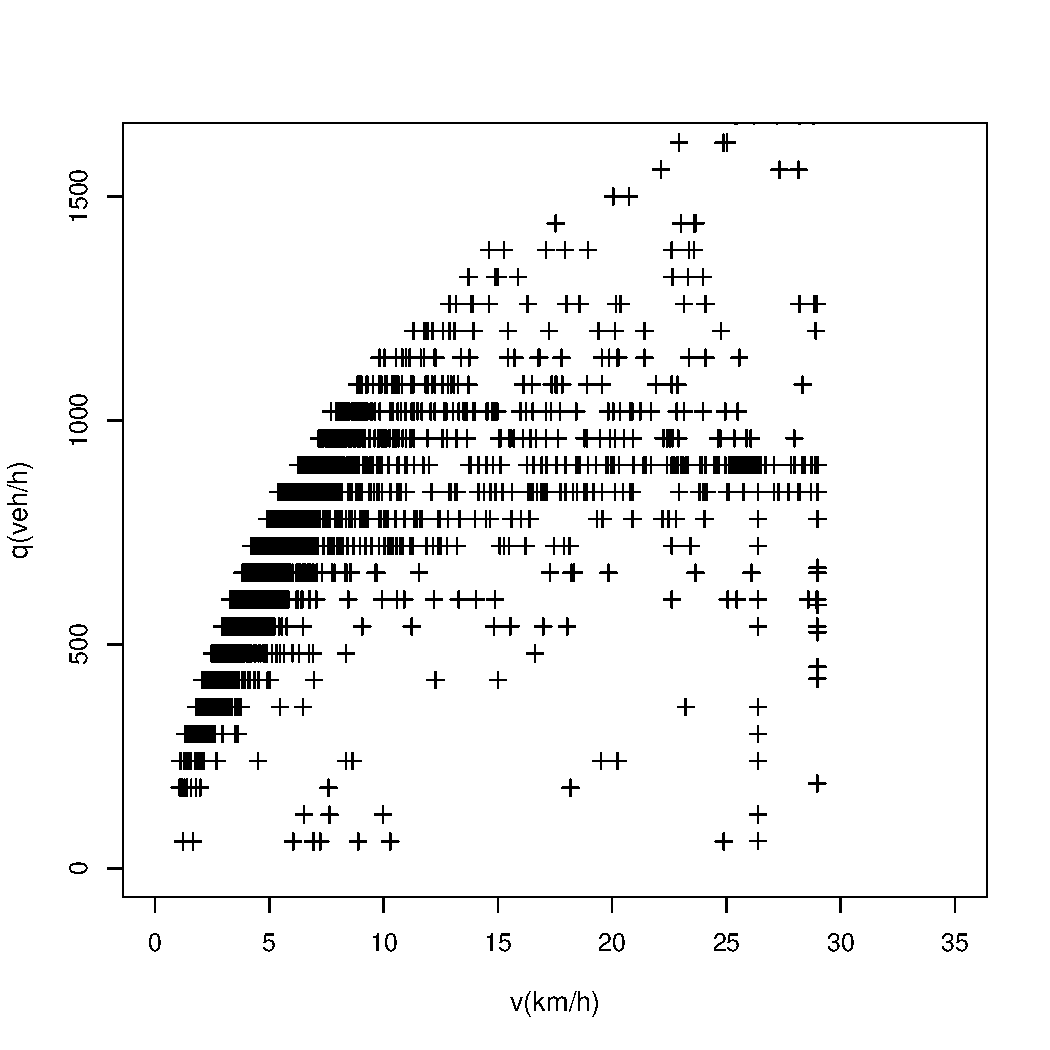
\includegraphics[width=0.33\linewidth]{factor2_vq_per25}}
\subfloat[][]{%
\label{factor2_vq_per50}%
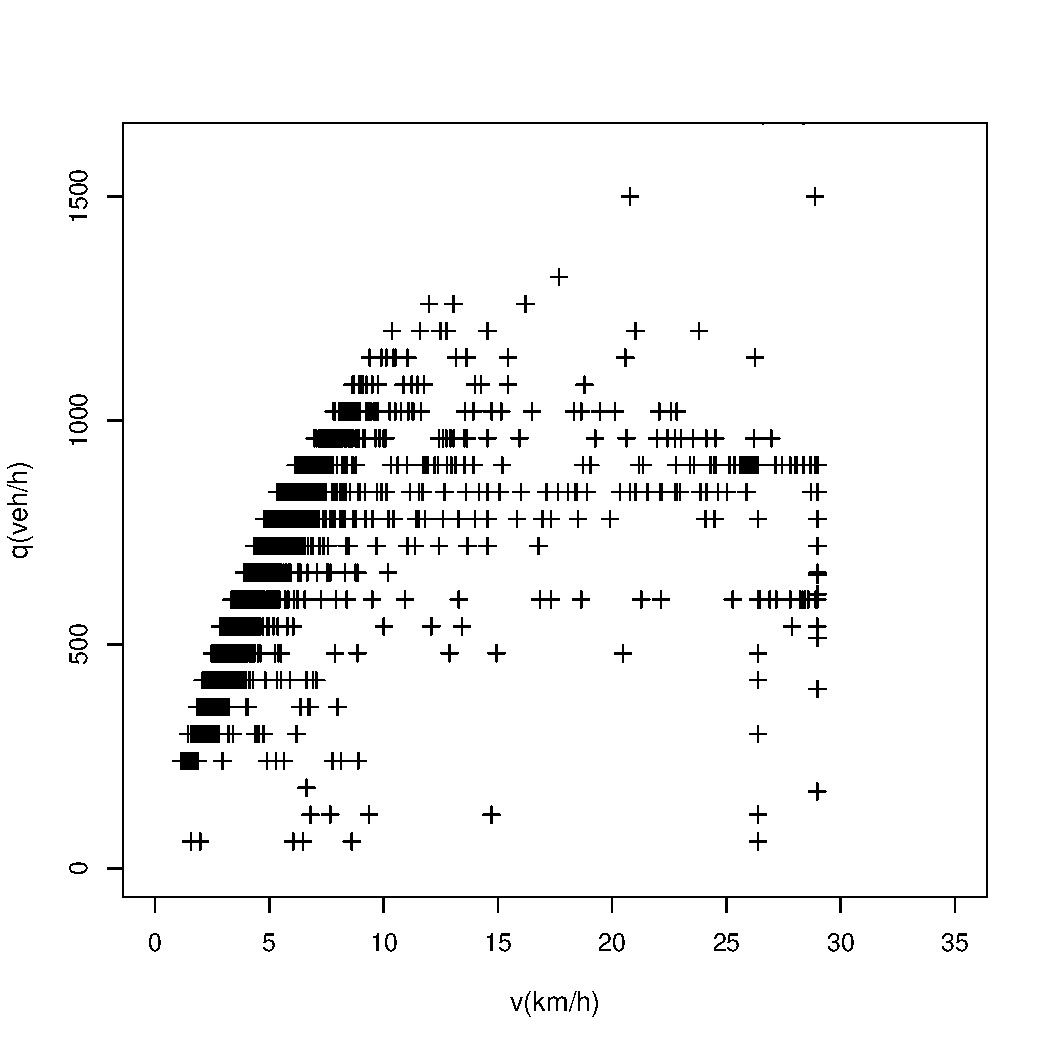
\includegraphics[width=0.33\linewidth]{factor2_vq_per50}}\\%
\subfloat[][]{%
\label{factor2_vq_per75}%
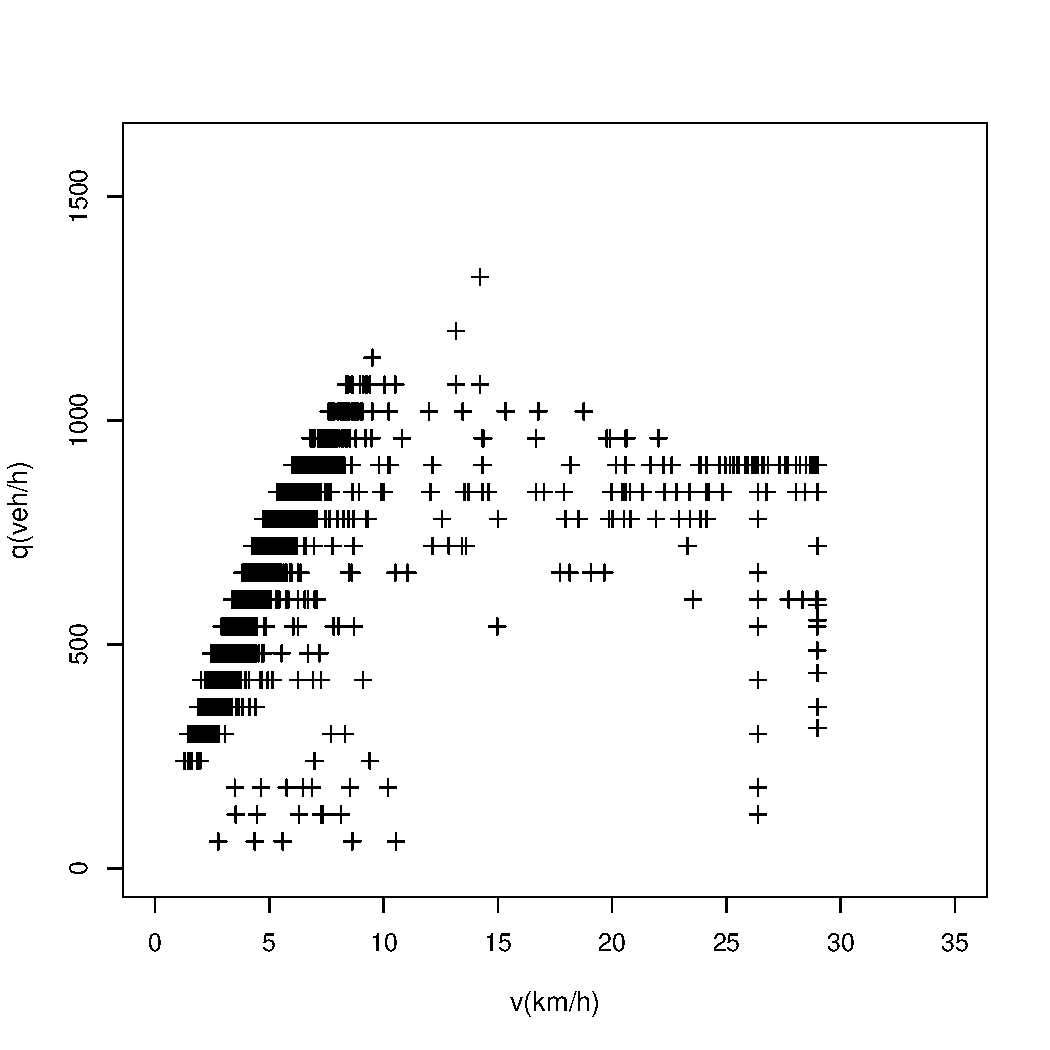
\includegraphics[width=0.33\linewidth]{factor2_vq_per75}}%
\subfloat[][]{%
\label{factor2_vq_per100}%
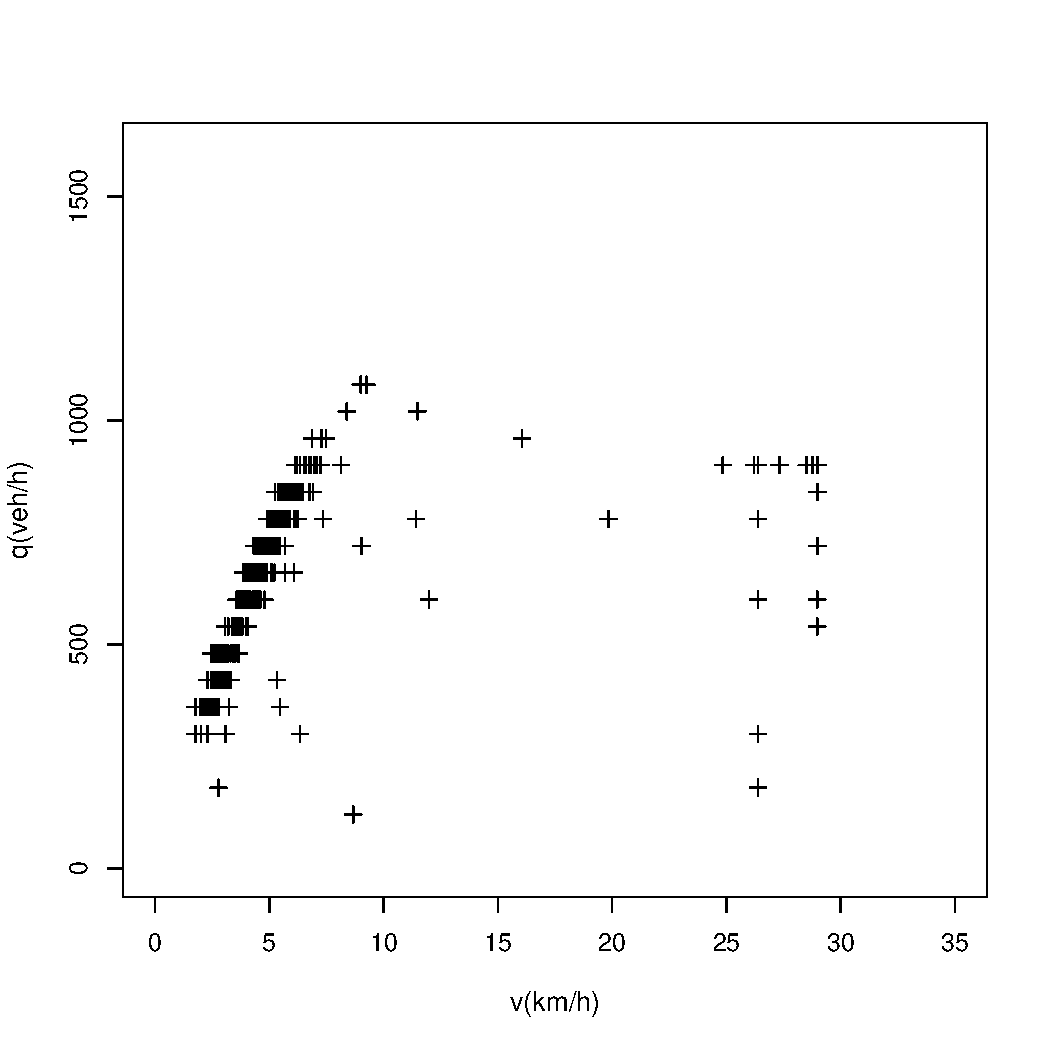
\includegraphics[width=0.33\linewidth]{factor2_vq_per100}}
\caption[A set of four sub-floats.]{最大减速度影响下速度流量关系图
\subref{factor2_vq_per0}
\subref{factor2_vq_per25} 
\subref{factor2_vq_per50}
\subref{factor2_vq_per75}
\subref{factor2_vq_per100}分别表示\autoref{decel-factor}中的B型驾驶人的百分比分别为0\%,25\%,50\%,75\%,100\%}%
\label{factor2_vq}%
\end{figure}



\begin{figure}[!htb]%
\centering
\subfloat[][]{
\label{factor2_kq_per0}%
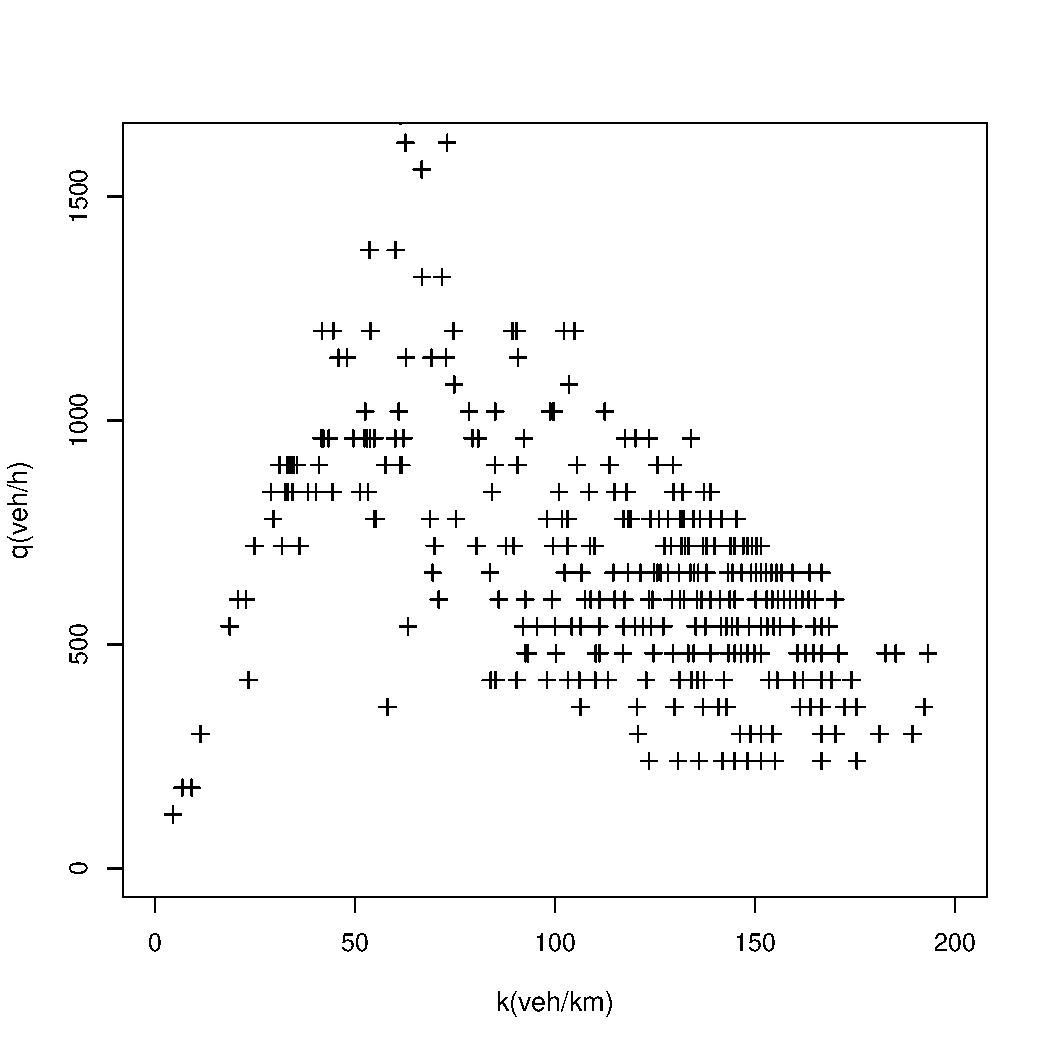
\includegraphics[width=0.33\linewidth]{factor2_kq_per0}
}%
\subfloat[][]{%
\label{factor2_kq_per25}%
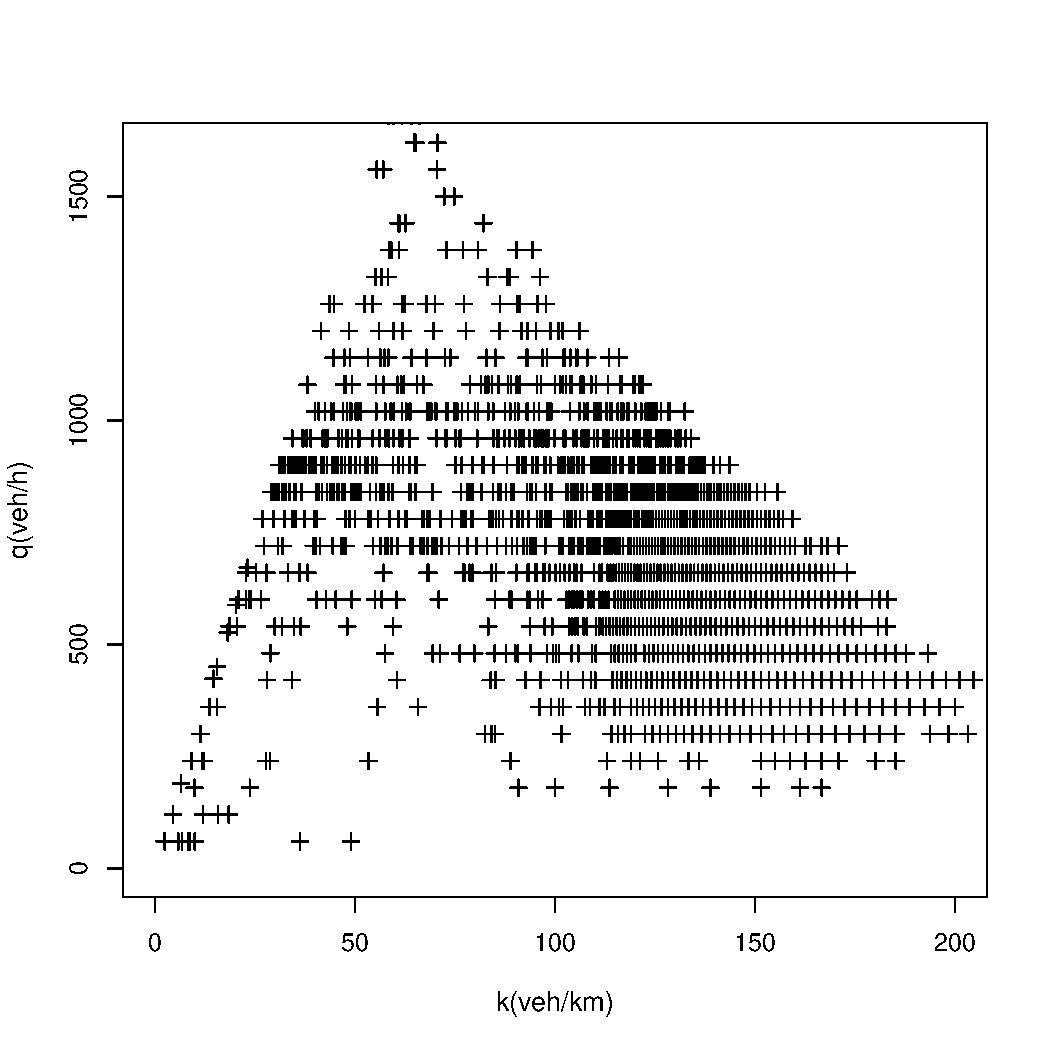
\includegraphics[width=0.33\linewidth]{factor2_kq_per25}}
\subfloat[][]{%
\label{factor2_kq_per50}%
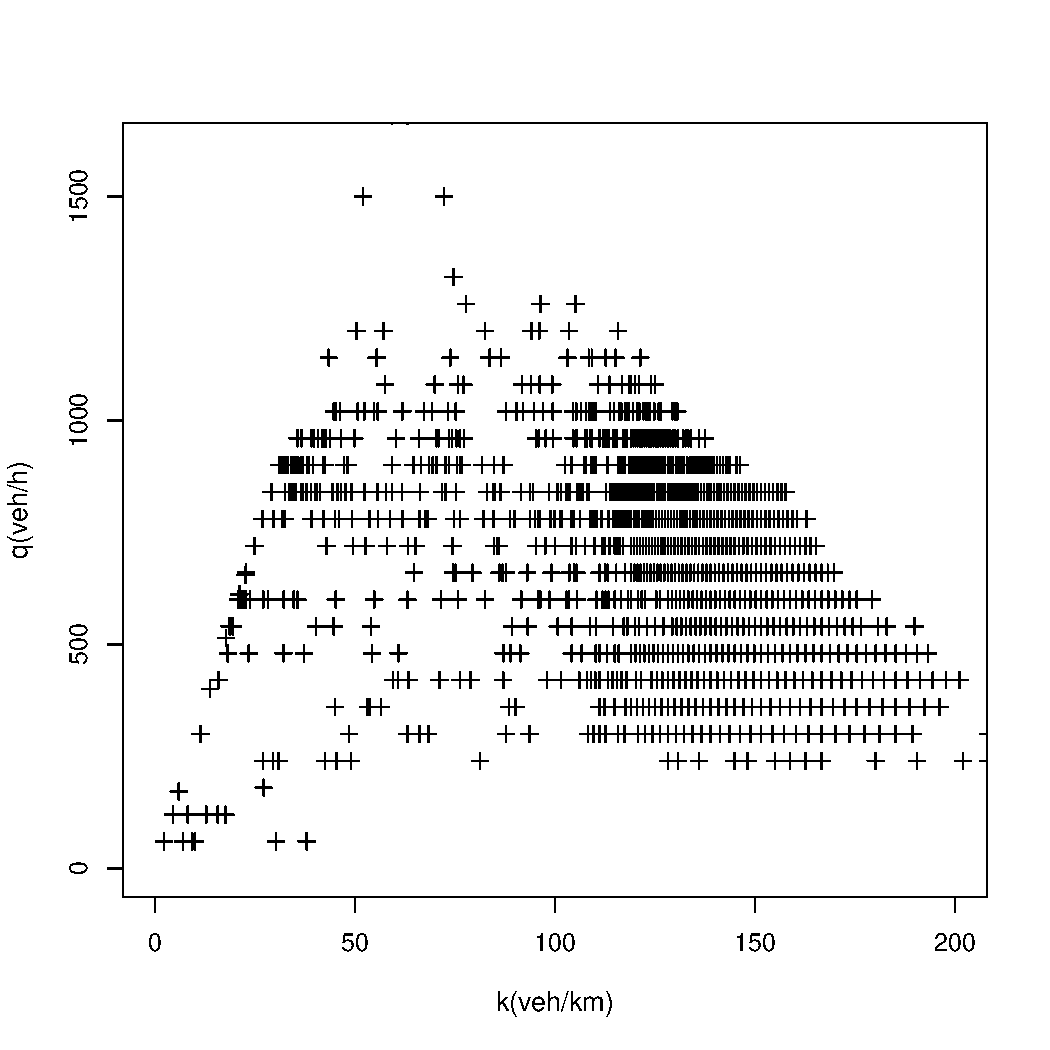
\includegraphics[width=0.33\linewidth]{factor2_kq_per50}}\\%
\subfloat[][]{%
\label{factor2_kq_per75}%
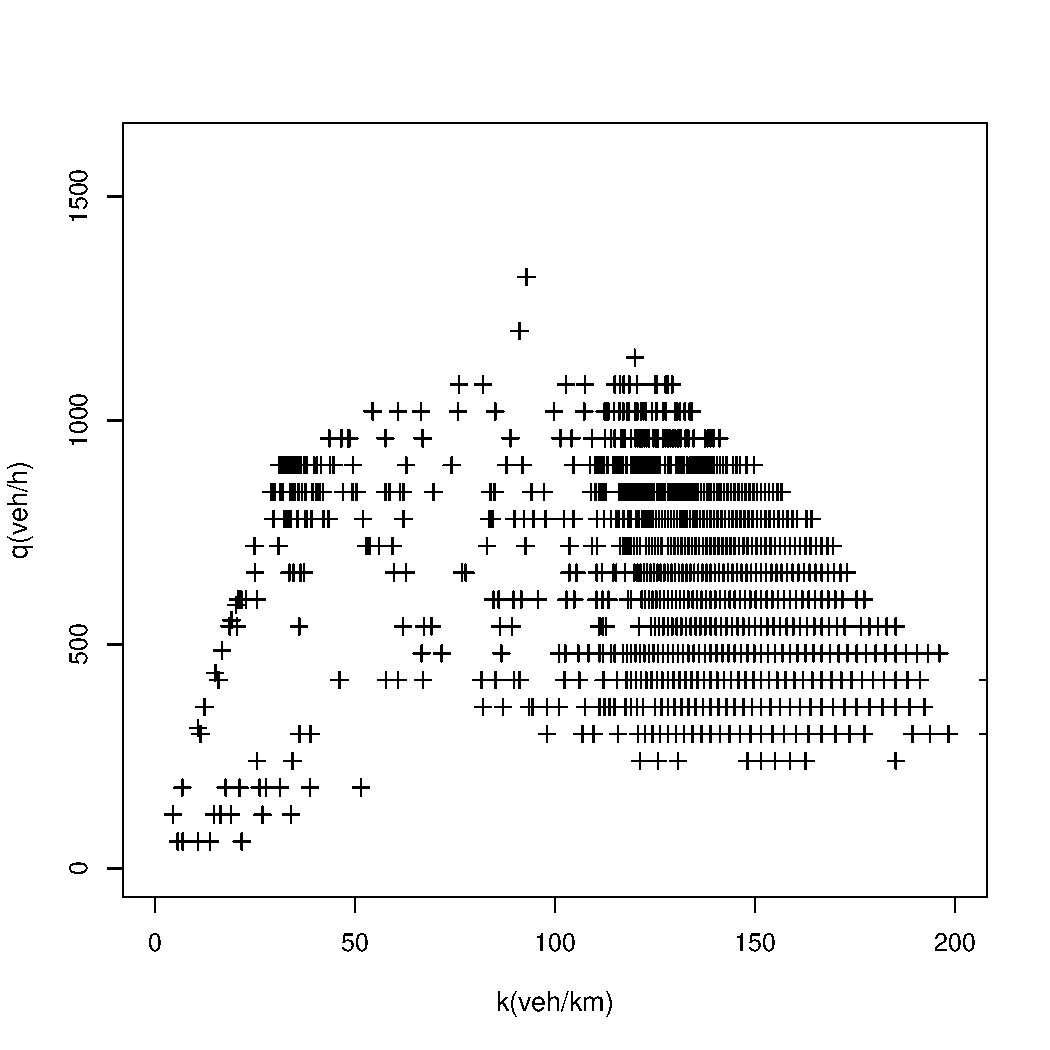
\includegraphics[width=0.33\linewidth]{factor2_kq_per75}}%
\subfloat[][]{%
\label{factor2_kq_per100}%
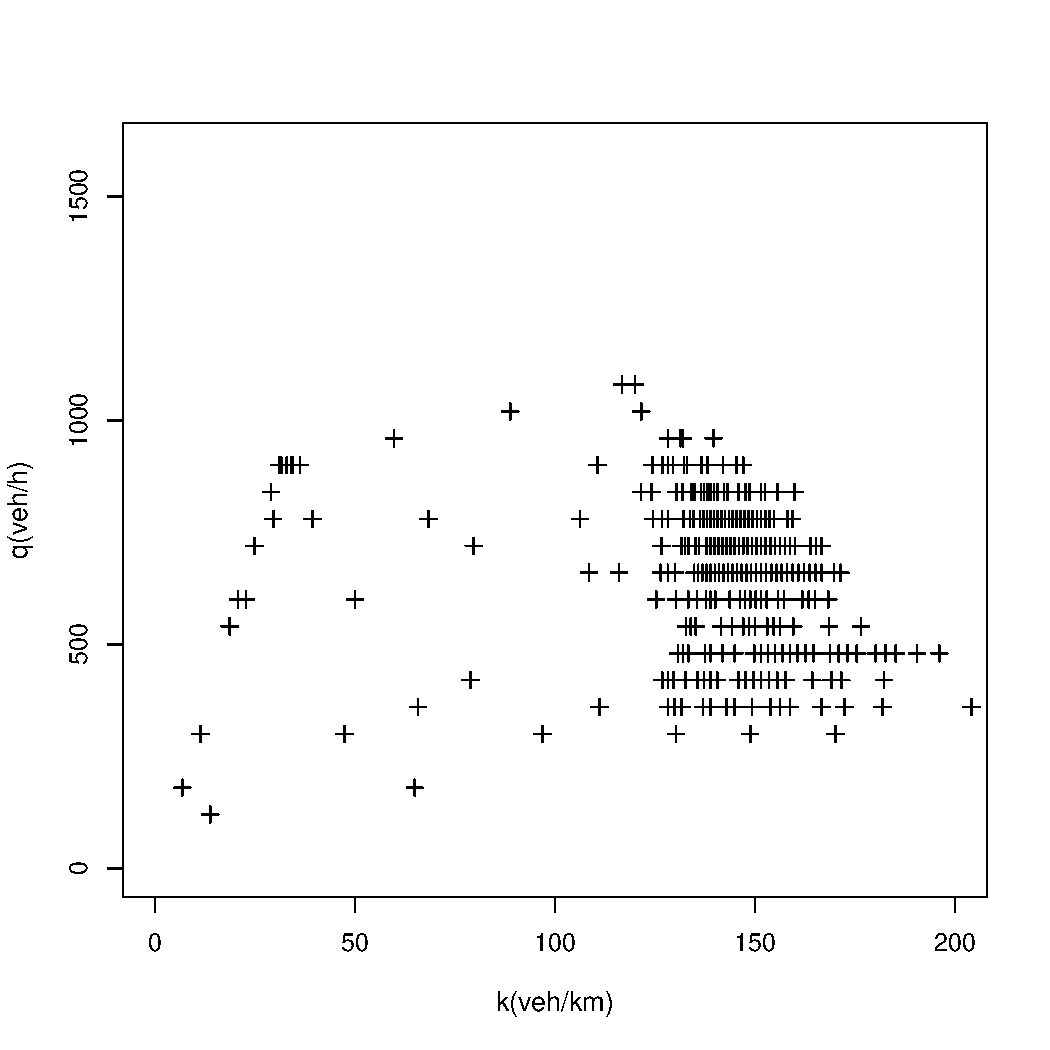
\includegraphics[width=0.33\linewidth]{factor2_kq_per100}}
\caption[A set of four sub-floats.]{最大减速度影响下的密度流量关系图
\subref{factor2_kq_per0}
\subref{factor2_kq_per25} 
\subref{factor2_kq_per50}
\subref{factor2_kq_per75}
\subref{factor2_kq_per100}分别表示\autoref{decel-factor}中的B型驾驶人的百分比分别为0\%,25\%,50\%,75\%,100\%}%
\label{factor2_kq}%
\end{figure}

\autoref{factor2_vq,factor2_kq}给出了,最大减速度影响下速度流量关系图和最大减速度影响下的密度流量关系图,可以看出,随着\autoref{decel-factor}中最大减速度较大的B型驾驶人的比例增加,在速度流量和密度流量关系图上均更难达到最大通行能力。这种趋势随着B型驾驶人的增加而更为明显。



\begin{figure}[!htb]
\begin{center}
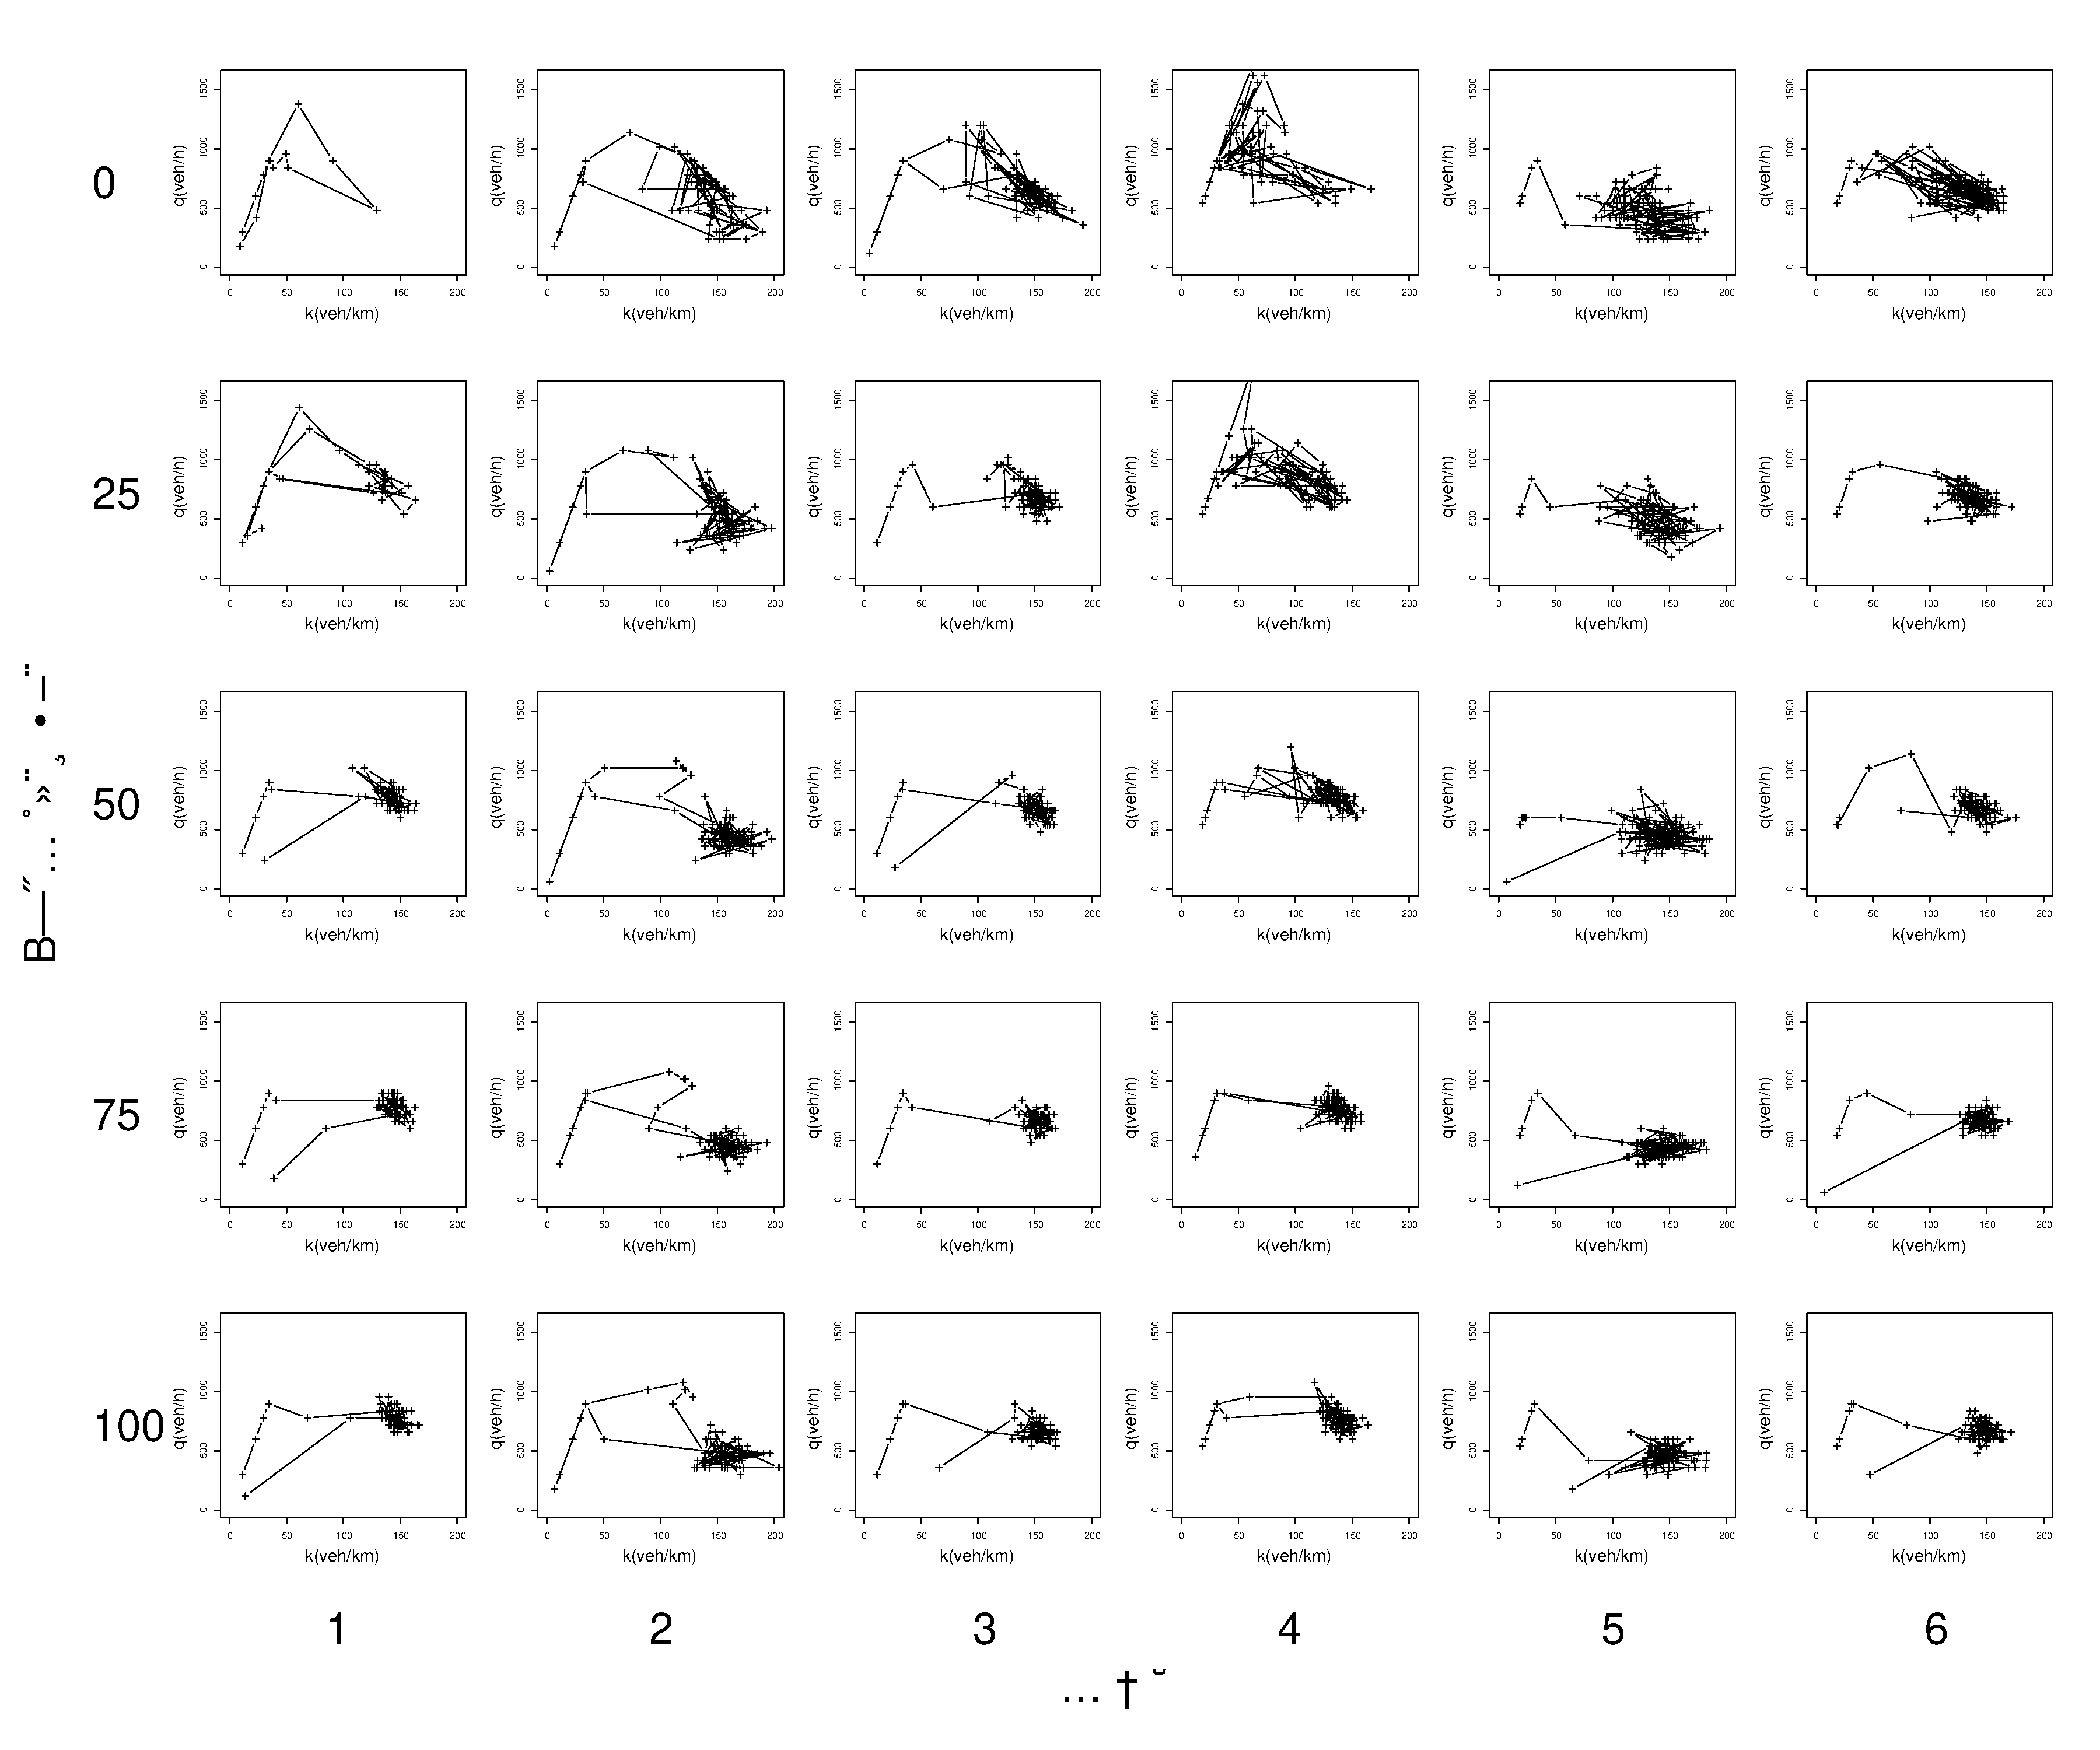
\includegraphics[width=\linewidth]{factor2_kqedges}
\caption{最大减速度影响下各检测器密度流量关系图}
\label{factor2_kqedges}
\end{center}
\end{figure}

最大减速度的增加造成密度流量图上,集中在J线以上,相对不稳定的状态。\autoref{factor2_kqedges}给出了最大减速度影响下各检测器密度流量关系图,从各检测器的密度流量状态跃迁图看,最为明显的是,检测器1和4的最大或接近最大通行能力,随着B型驾驶人的更多的混入,从自由流的状态更多的往同步流状态跃迁。


\subsection{混合影响因素}

\autoref{combined_box_ttime}\autoref{combined_vq}\autoref{combined_kq}\autoref{combined_kqedges},分别给出了混合作用影响下模拟用时箱图,速度流量关系图,密度流量关系图和各检测器密度流量关系图。其结果与最大减速度影响下的结果相似,可以推断对交通流斜率新的影响,主要的贡献成分来自于最大减速度的影响,最大减速度越大则交通流越难达到最大通行能力,也越多的处于较为不稳定的同步流状态。

\begin{figure}[!htb]
\begin{center}
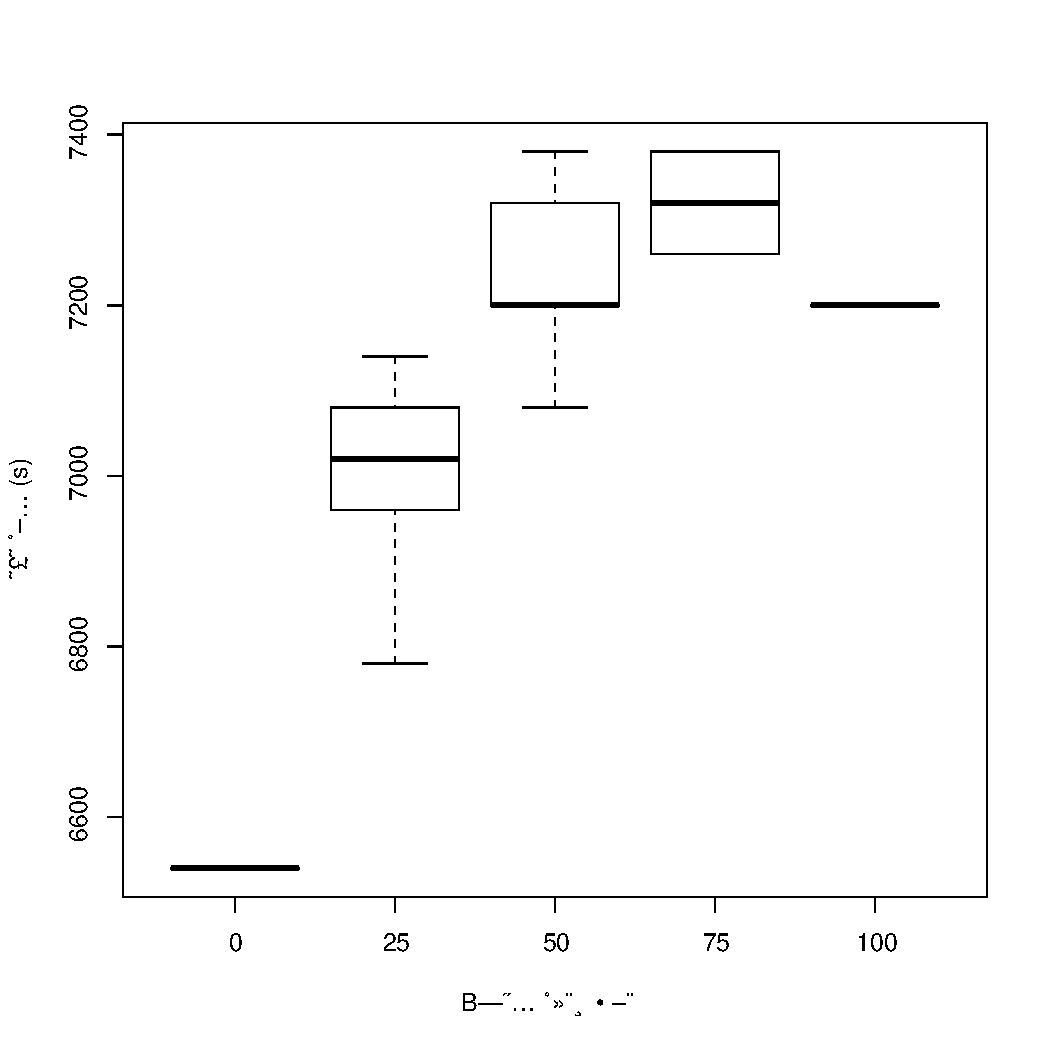
\includegraphics[width=0.5\linewidth]{combined_box_ttime}
\label{combined_box_ttime}
\caption{混合作用影响下模拟用时箱图}
\end{center}
\end{figure}



\begin{figure}[!htb]%
\centering
\subfloat[][]{
\label{combined_vq_per0}%
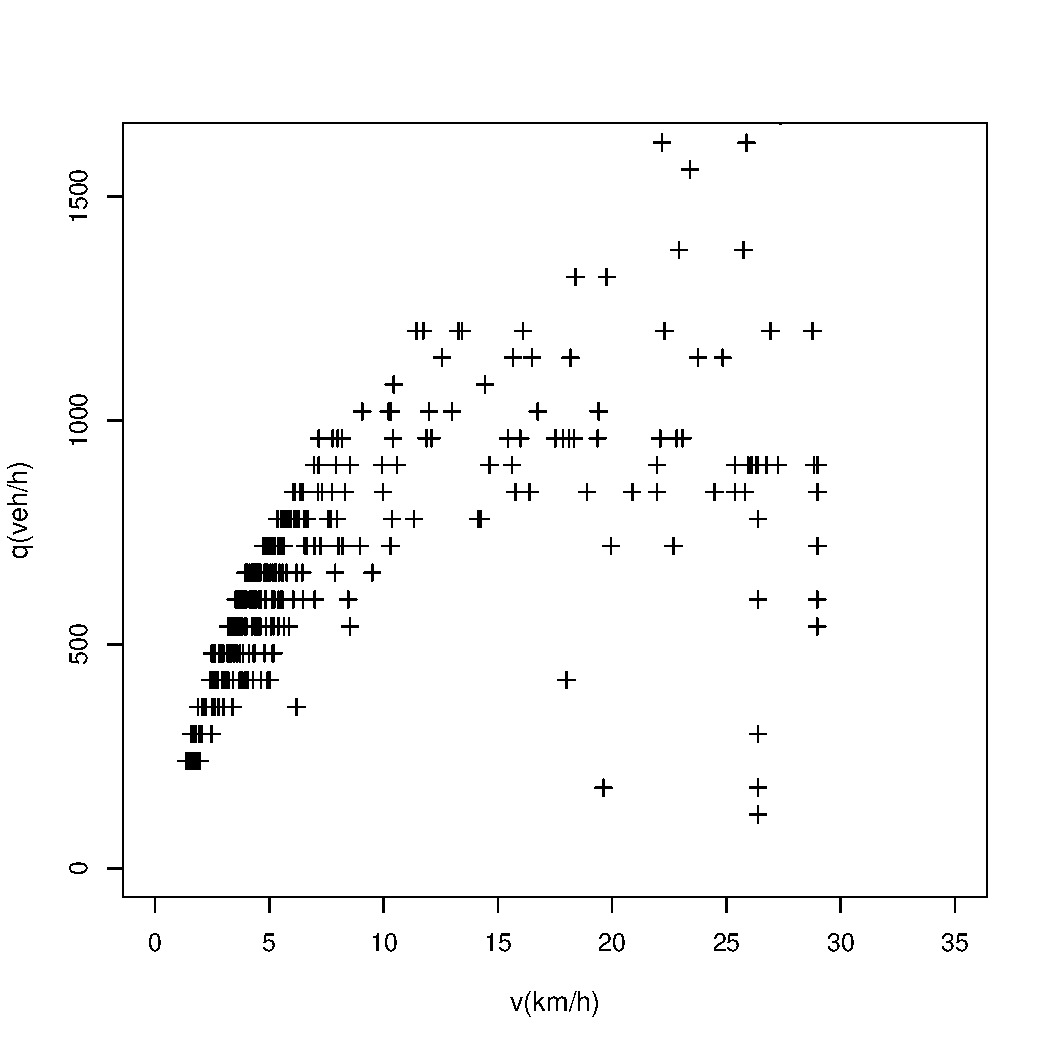
\includegraphics[width=0.33\linewidth]{combined_vq_per0}
}%
\subfloat[][]{%
\label{combined_vq_per25}%
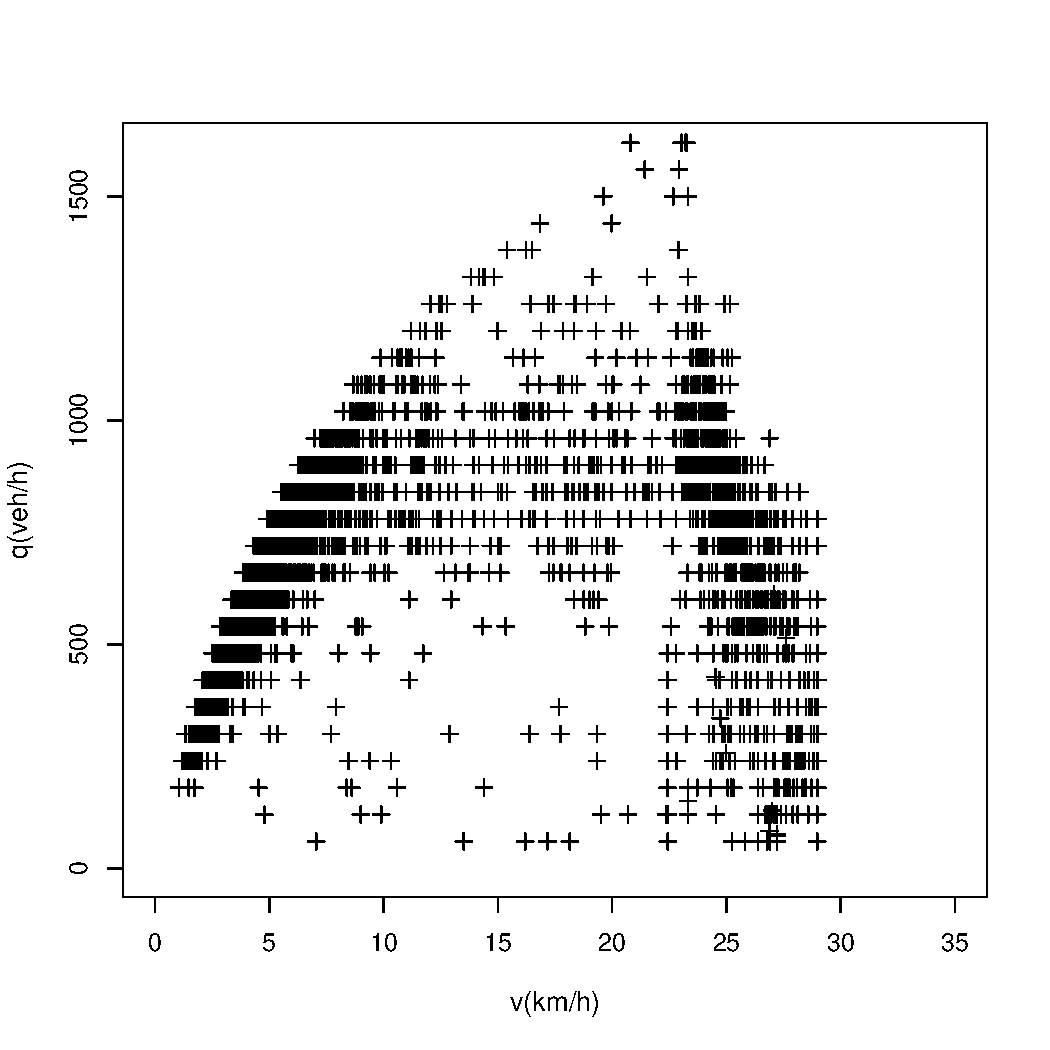
\includegraphics[width=0.33\linewidth]{combined_vq_per25}}
\subfloat[][]{%
\label{combined_vq_per50}%
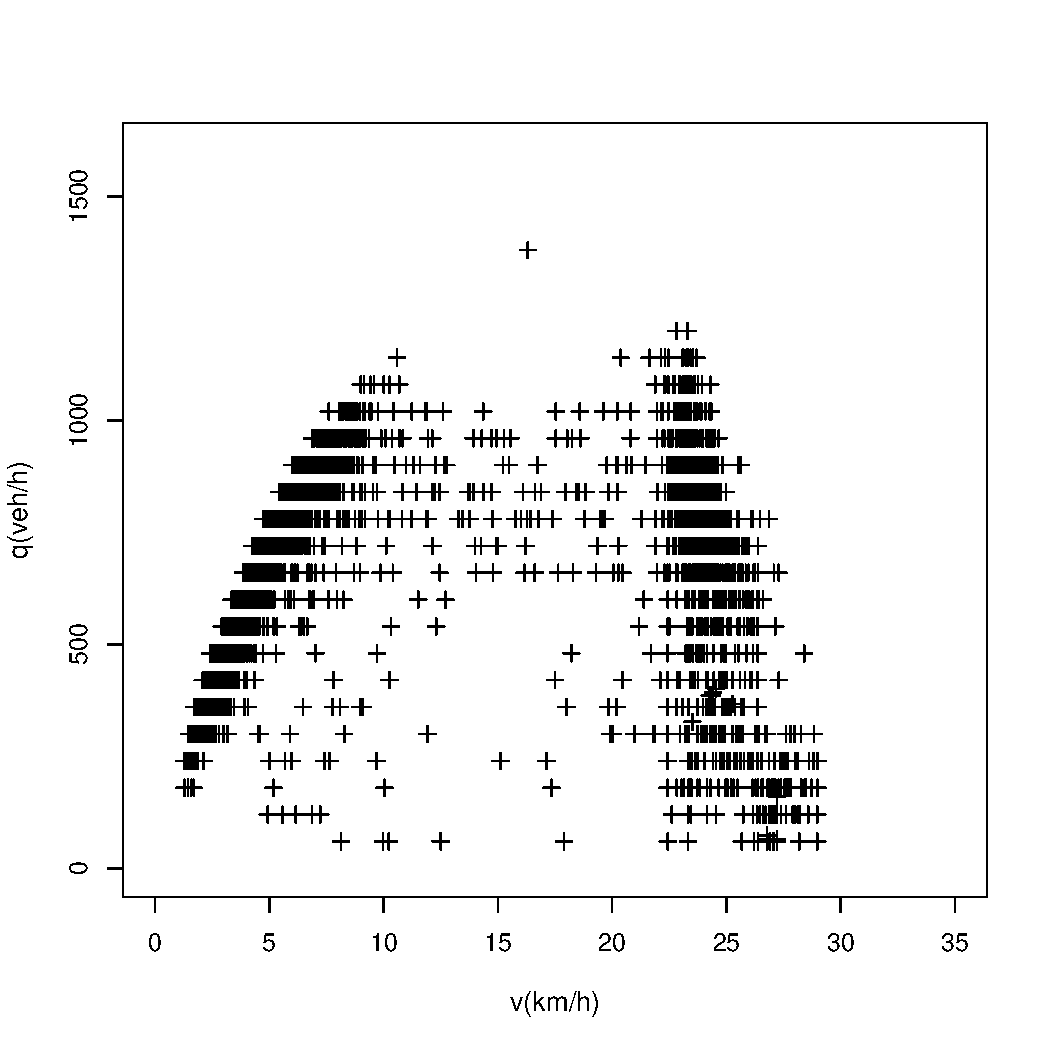
\includegraphics[width=0.33\linewidth]{combined_vq_per50}}\\%
\subfloat[][]{%
\label{combined_vq_per75}%
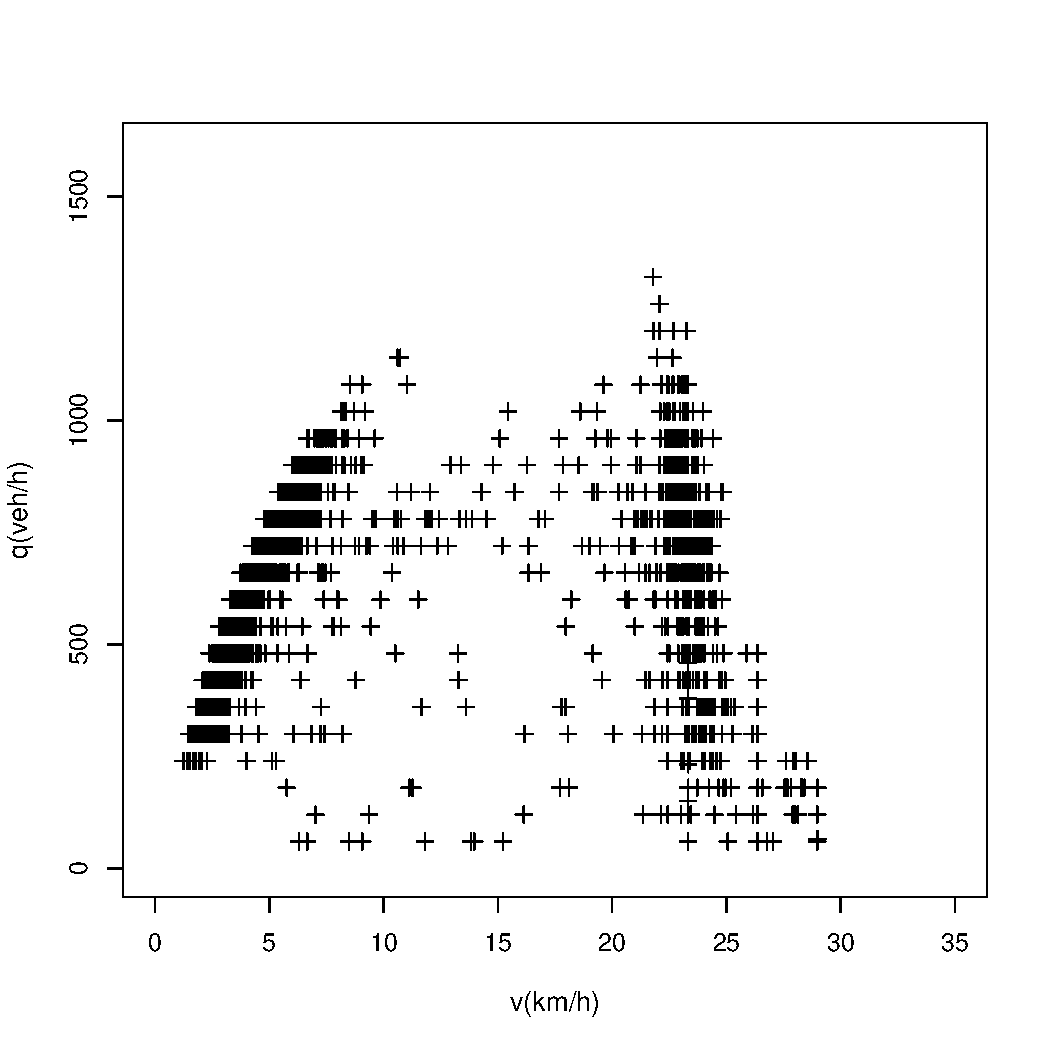
\includegraphics[width=0.33\linewidth]{combined_vq_per75}}%
\subfloat[][]{%
\label{combined_vq_per100}%
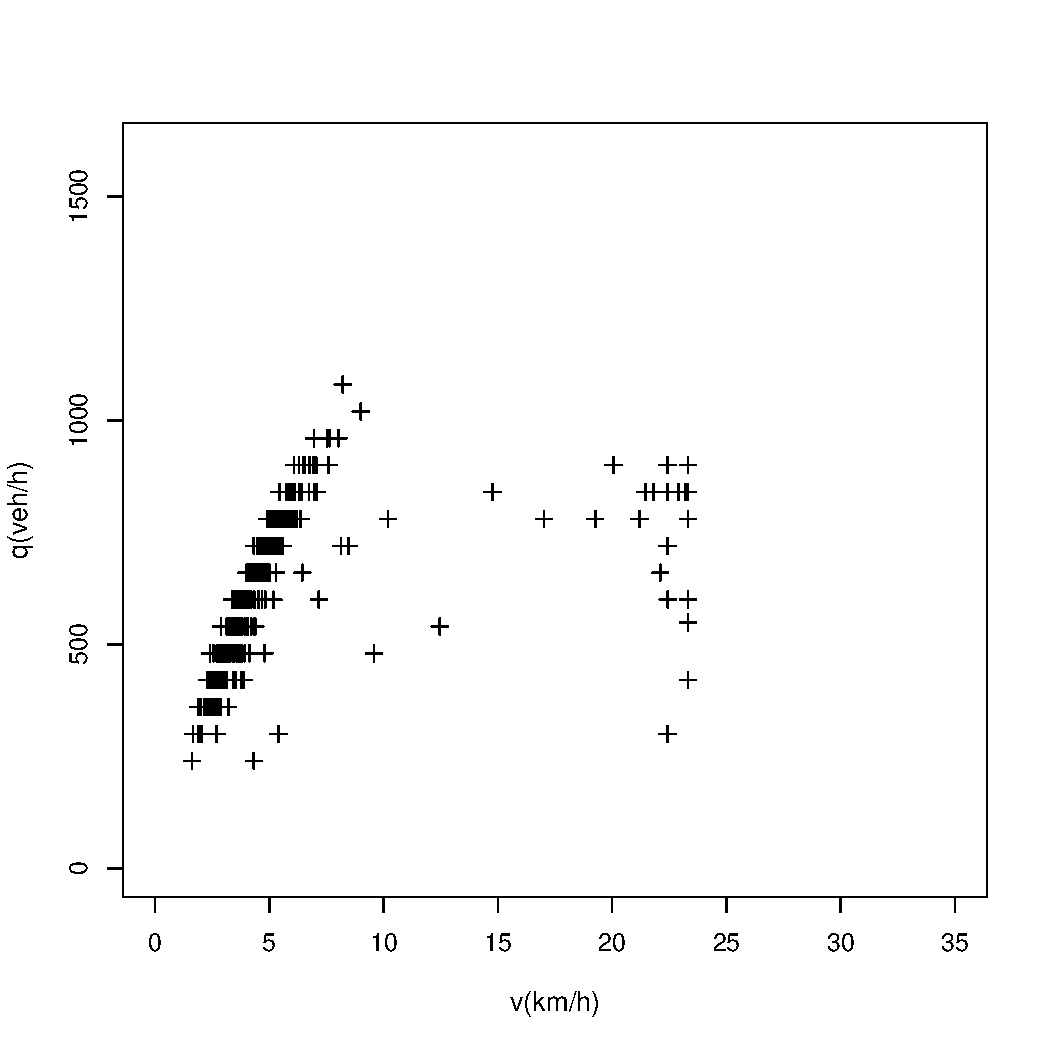
\includegraphics[width=0.33\linewidth]{combined_vq_per100}}
\caption[A set of four sub-floats.]{混合作用影响下速度流量关系图
\subref{combined_vq_per0}
\subref{combined_vq_per25} 
\subref{combined_vq_per50}
\subref{combined_vq_per75}
\subref{combined_vq_per100}分别表示\autoref{combined-factor}中的B型驾驶人的百分比分别为0\%,25\%,50\%,75\%,100\%}%
\label{combined_vq}%
\end{figure}


\begin{figure}[!htb]%
\centering
\subfloat[][]{
\label{combined_kq_per0}%
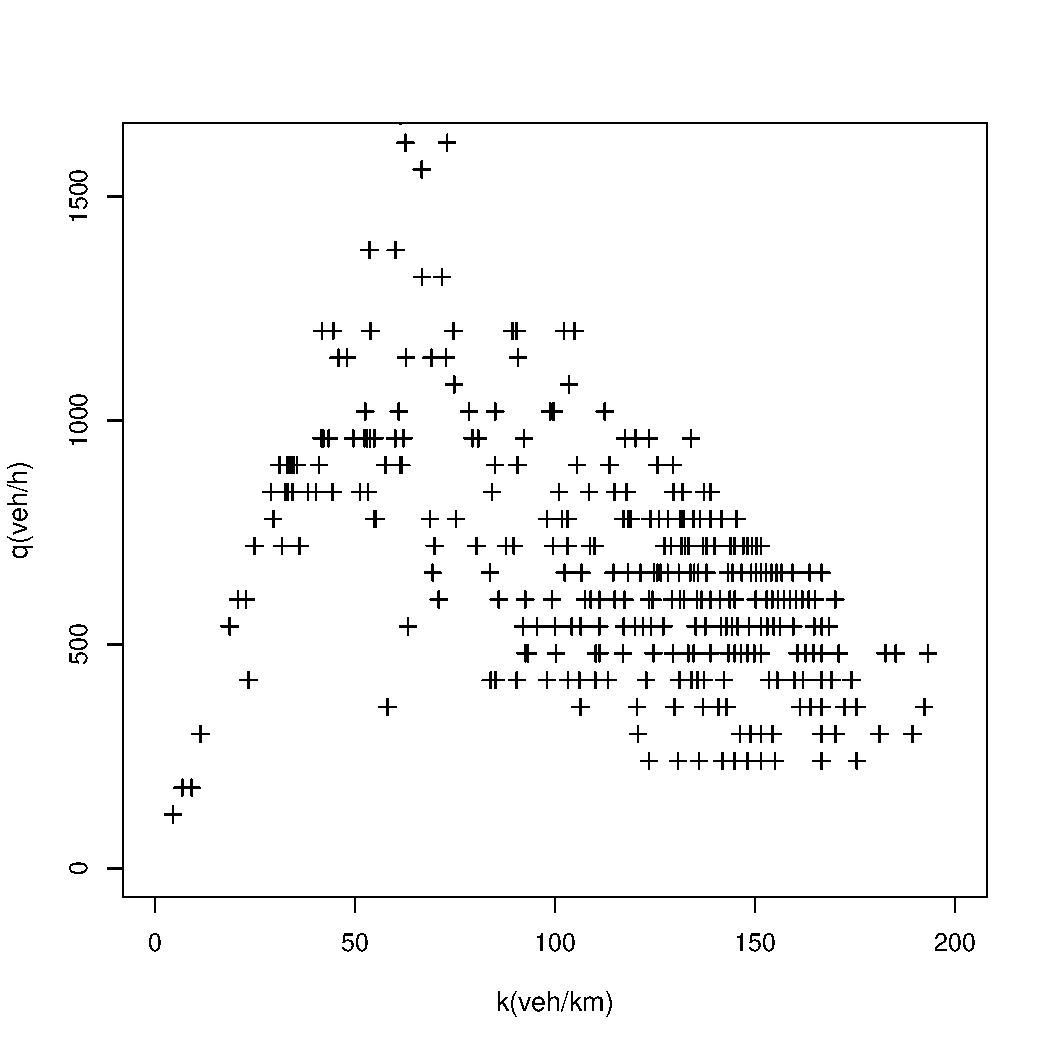
\includegraphics[width=0.33\linewidth]{combined_kq_per0}
}%
\subfloat[][]{%
\label{combined_kq_per25}%
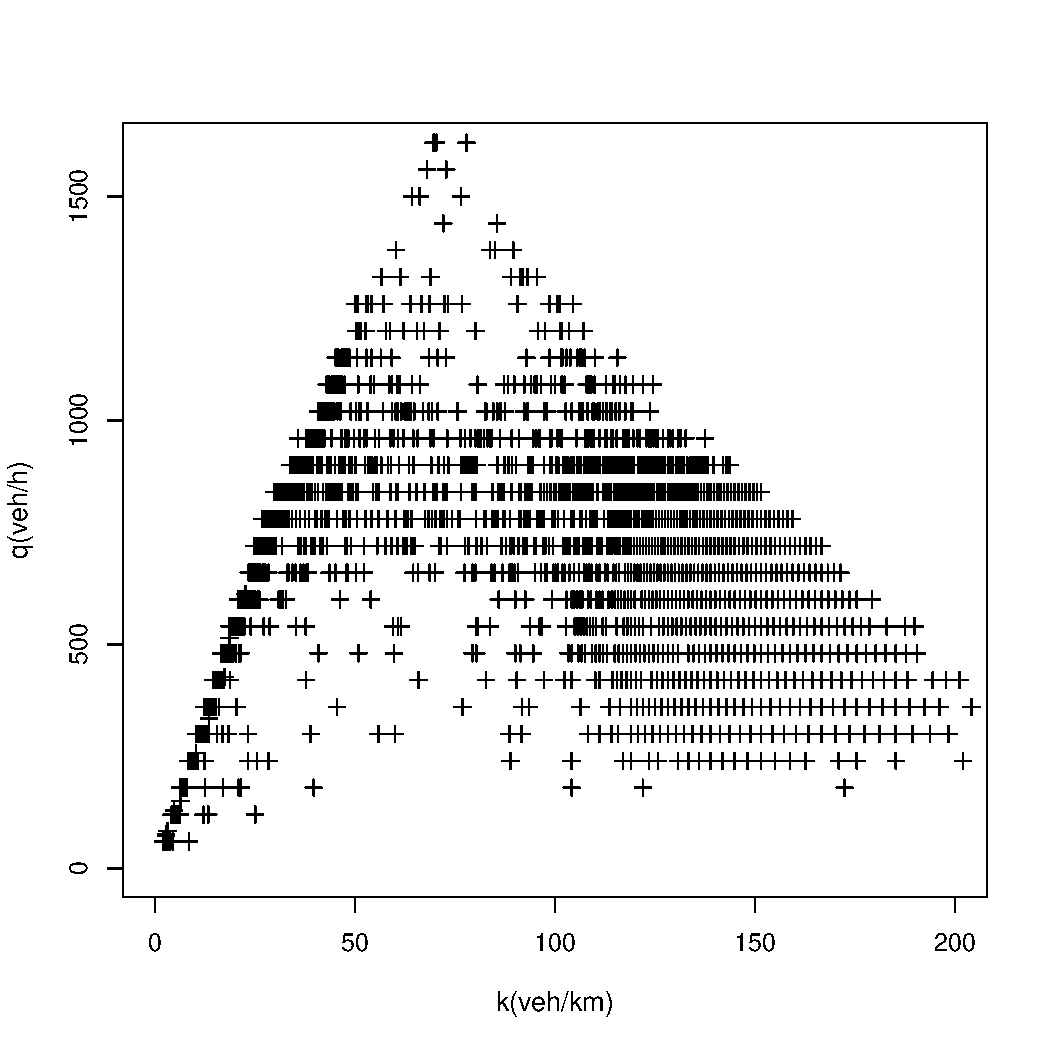
\includegraphics[width=0.33\linewidth]{combined_kq_per25}}
\subfloat[][]{%
\label{combined_kq_per50}%
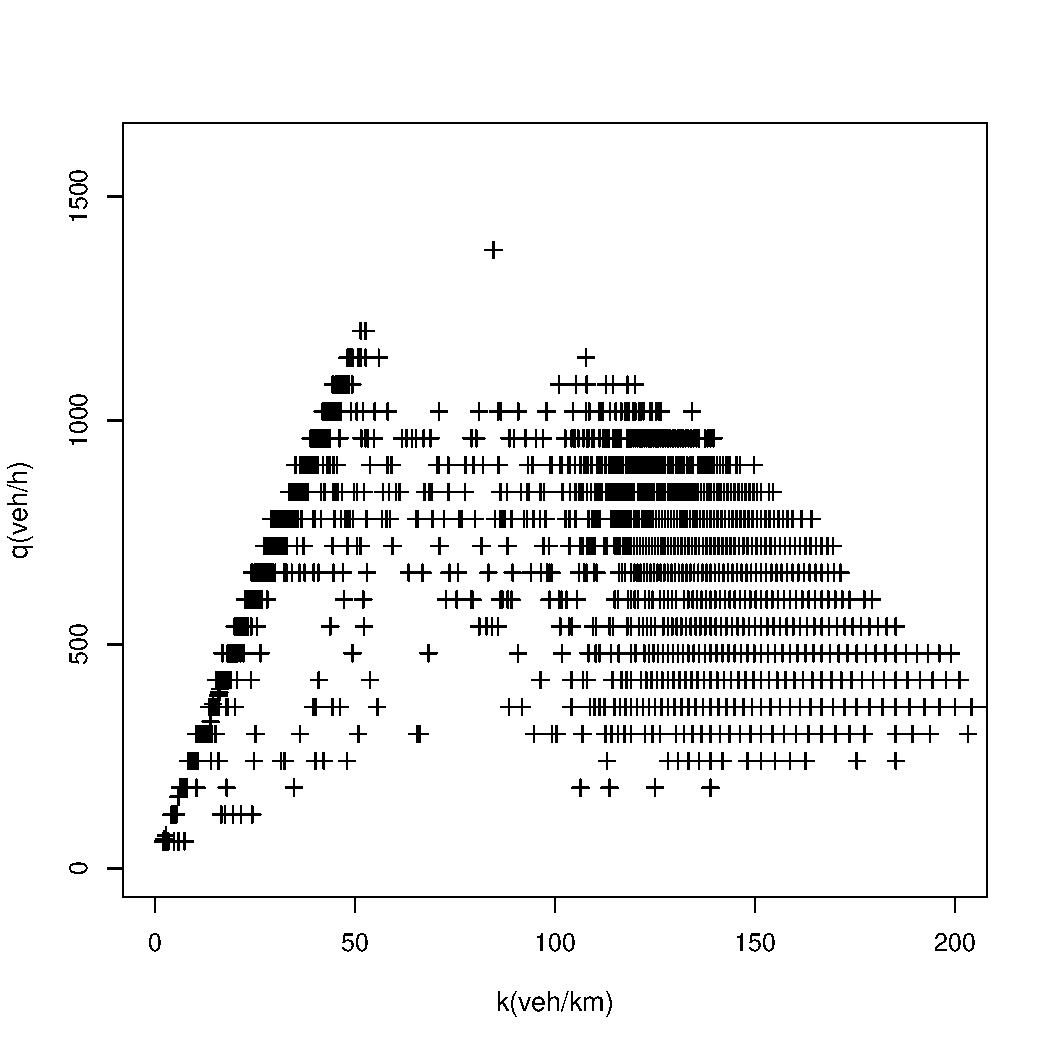
\includegraphics[width=0.33\linewidth]{combined_kq_per50}}\\%
\subfloat[][]{%
\label{combined_kq_per75}%
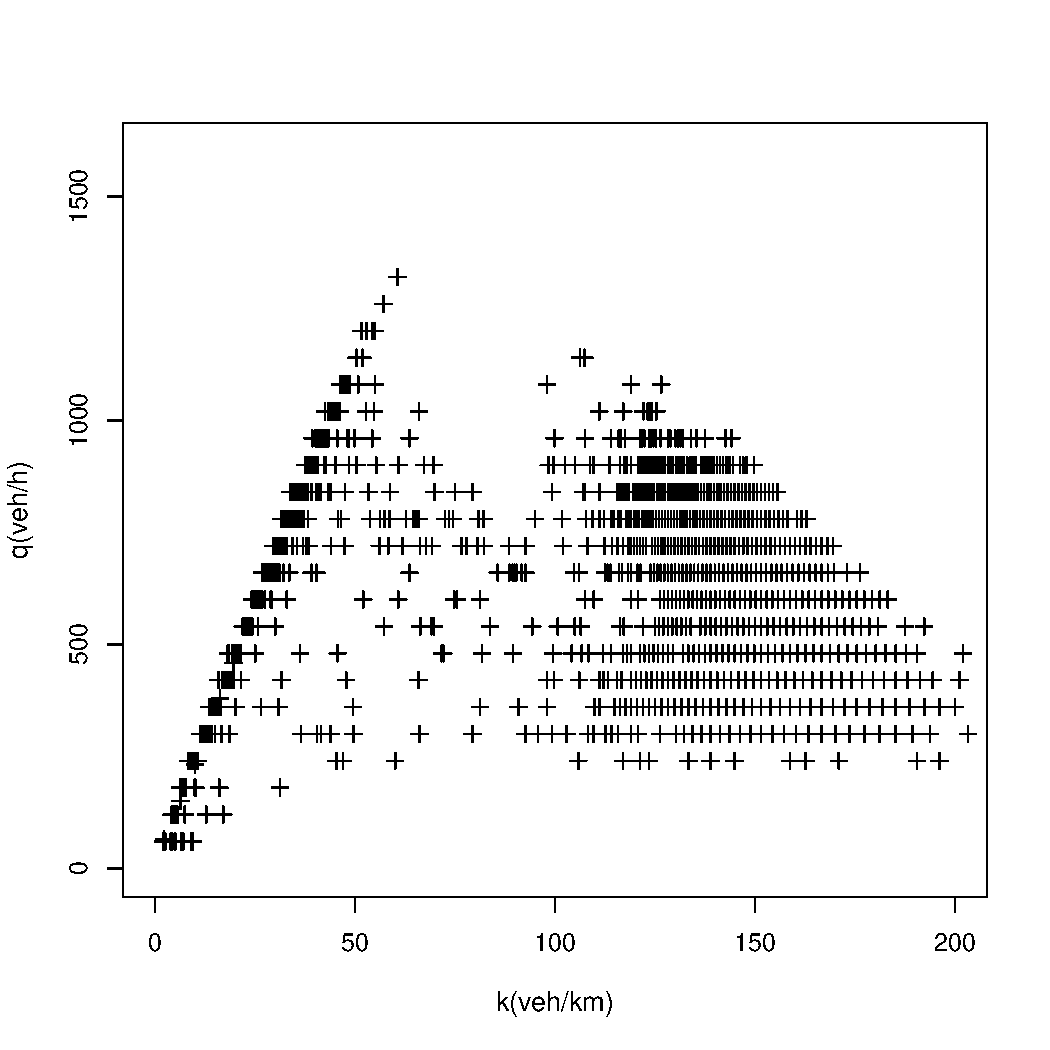
\includegraphics[width=0.33\linewidth]{combined_kq_per75}}%
\subfloat[][]{%
\label{combined_kq_per100}%
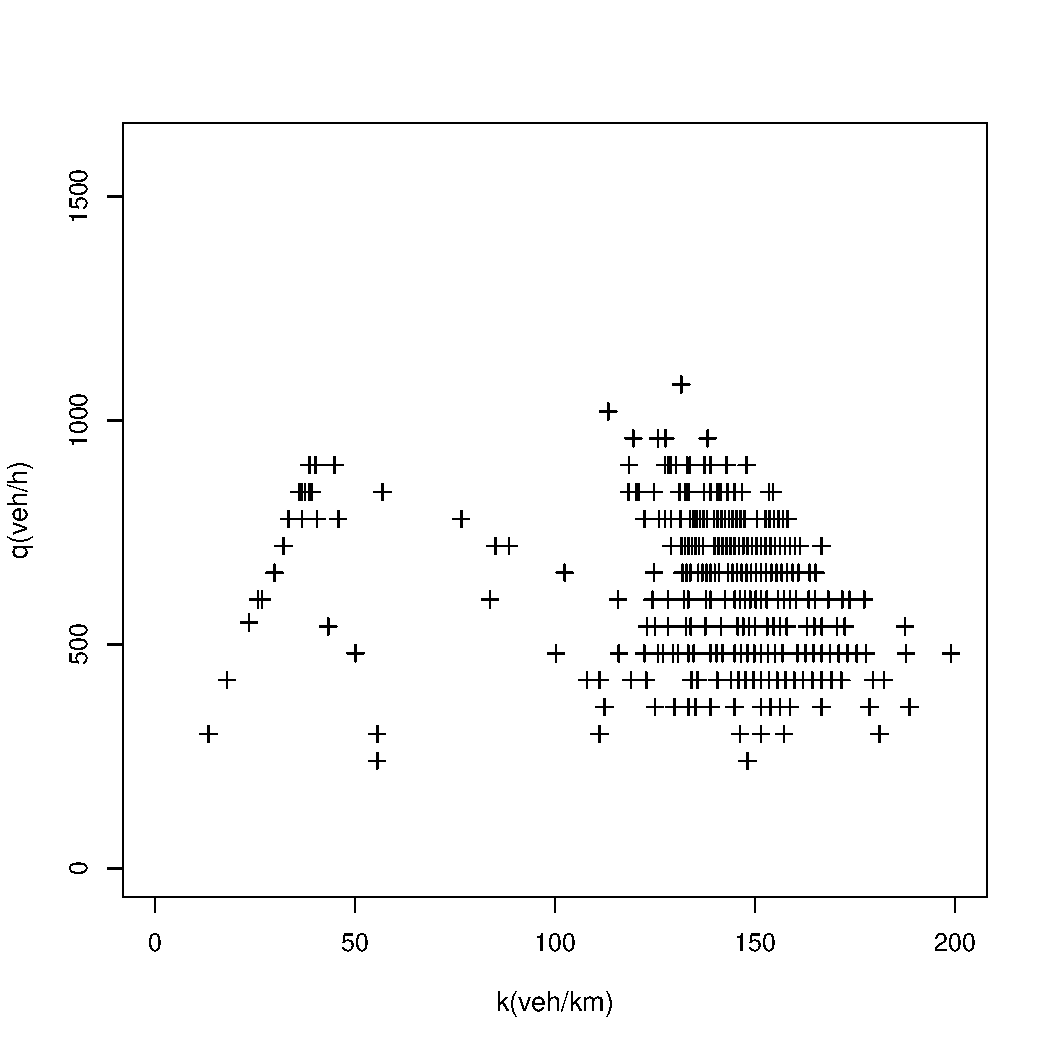
\includegraphics[width=0.33\linewidth]{combined_kq_per100}}
\caption[A set of four sub-floats.]{混合作用影响下的密度流量关系图
\subref{combined_kq_per0}
\subref{combined_kq_per25} 
\subref{combined_kq_per50}
\subref{combined_kq_per75}
\subref{combined_kq_per100}分别表示\autoref{combined-factor}中的B型驾驶人的百分比分别为0\%,25\%,50\%,75\%,100\%}%
\label{combined_kq}%
\end{figure}

\begin{figure}[!htb]
\begin{center}
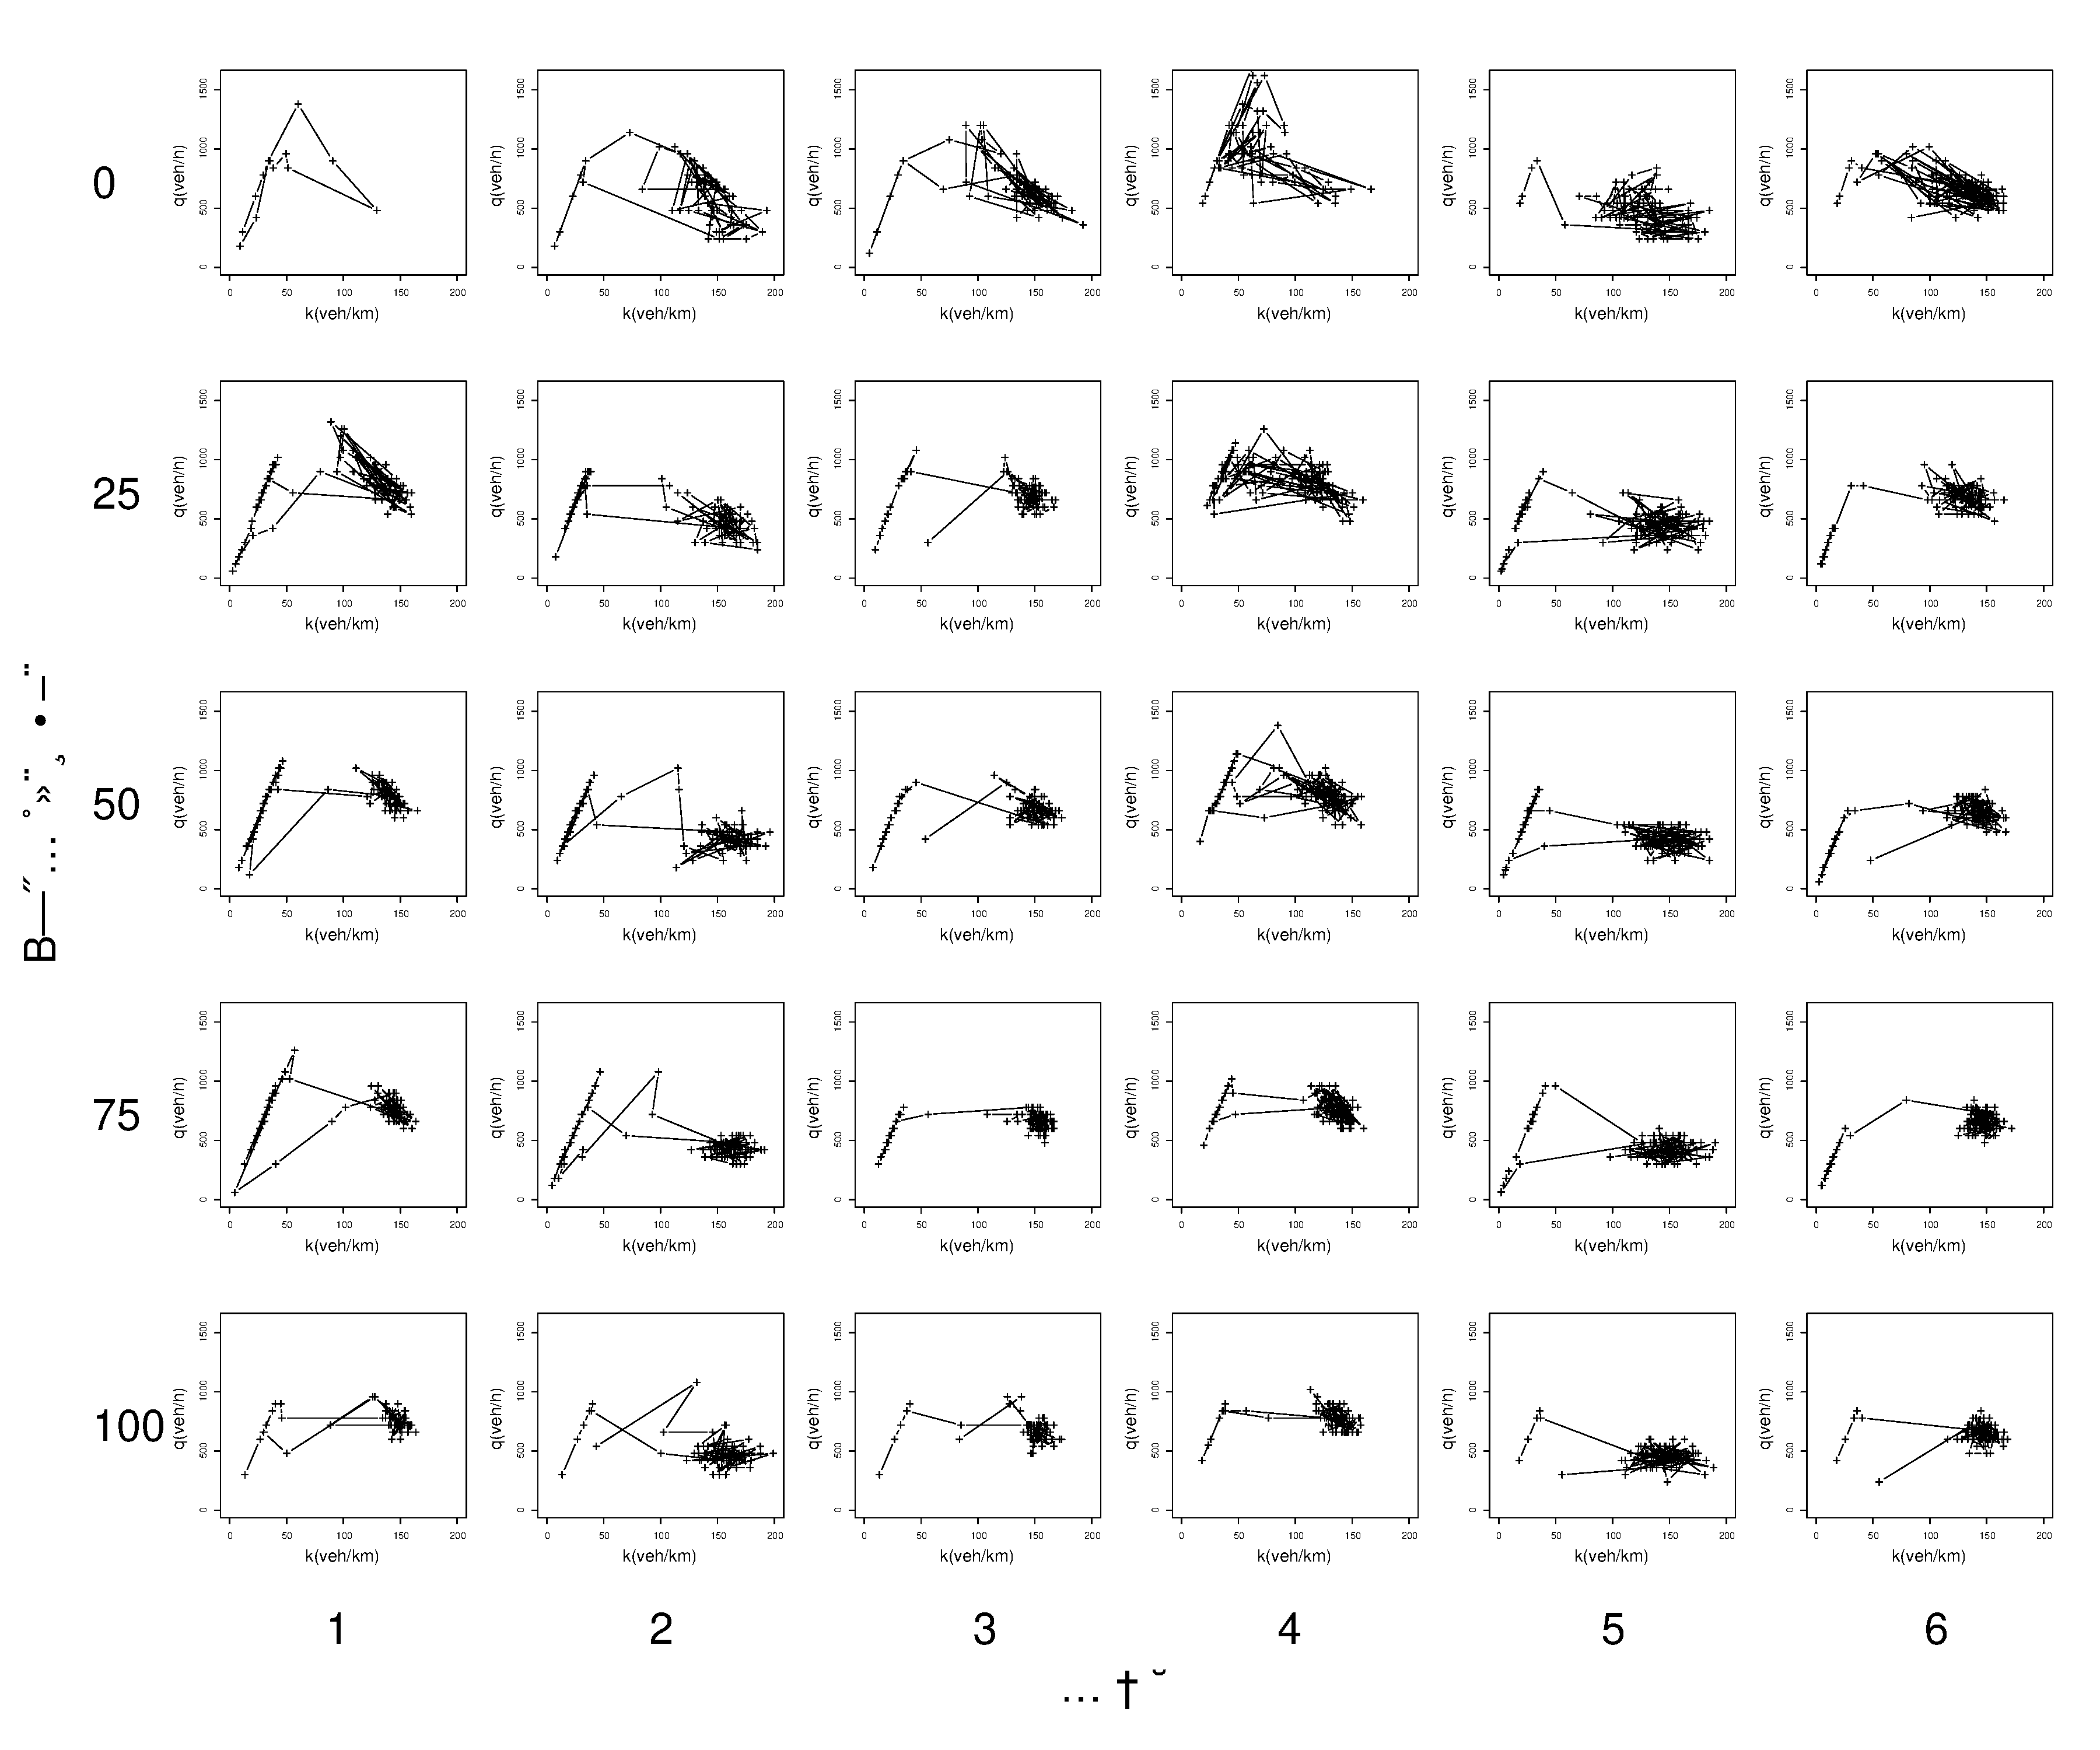
\includegraphics[width=\linewidth]{combined_kqedges}
\caption{混合作用影响下各检测器密度流量关系图}
\label{combined_kqedges}
\end{center}
\end{figure}

\section{对交通流安全性}

评价交通流安全性,使用了TTC倒数的一分钟和值,以及6个检测器流量的一分钟平均值。

TTC倒数的时间平均产生密度,

\subsection{期望速度影响因素}

期望速度从\autoref{factor1_ttc}流量与TTC倒数关系图看,TTC倒数的和值的绝对值最大主要出现在流量600-800之间,从图上看对其分布没有显著影响。由\autoref{factor1_box_avttc}可以看出,期望车速对,时间平均TTC倒数(或者说TTC倒数的时间产生密度)的绝对值有显著的影响,随着期望车速较高的B型驾驶人更多的混入,时间平均TTC倒数的绝对值呈现增加的趋势。当B型驾驶人的比例小于50\%时,使用不同随机数的情况差异较大,说明车辆的顺序对时间平均TTC倒数产生显著的影响。可以理解为低期望车速阻碍高期望车速的作用在B型驾驶人较少时,对交通流的安全性产生较大增加随机性的影响。

\begin{figure}[!htb]%
\centering
\subfloat[][]{
\label{factor1_ttc_per0}%
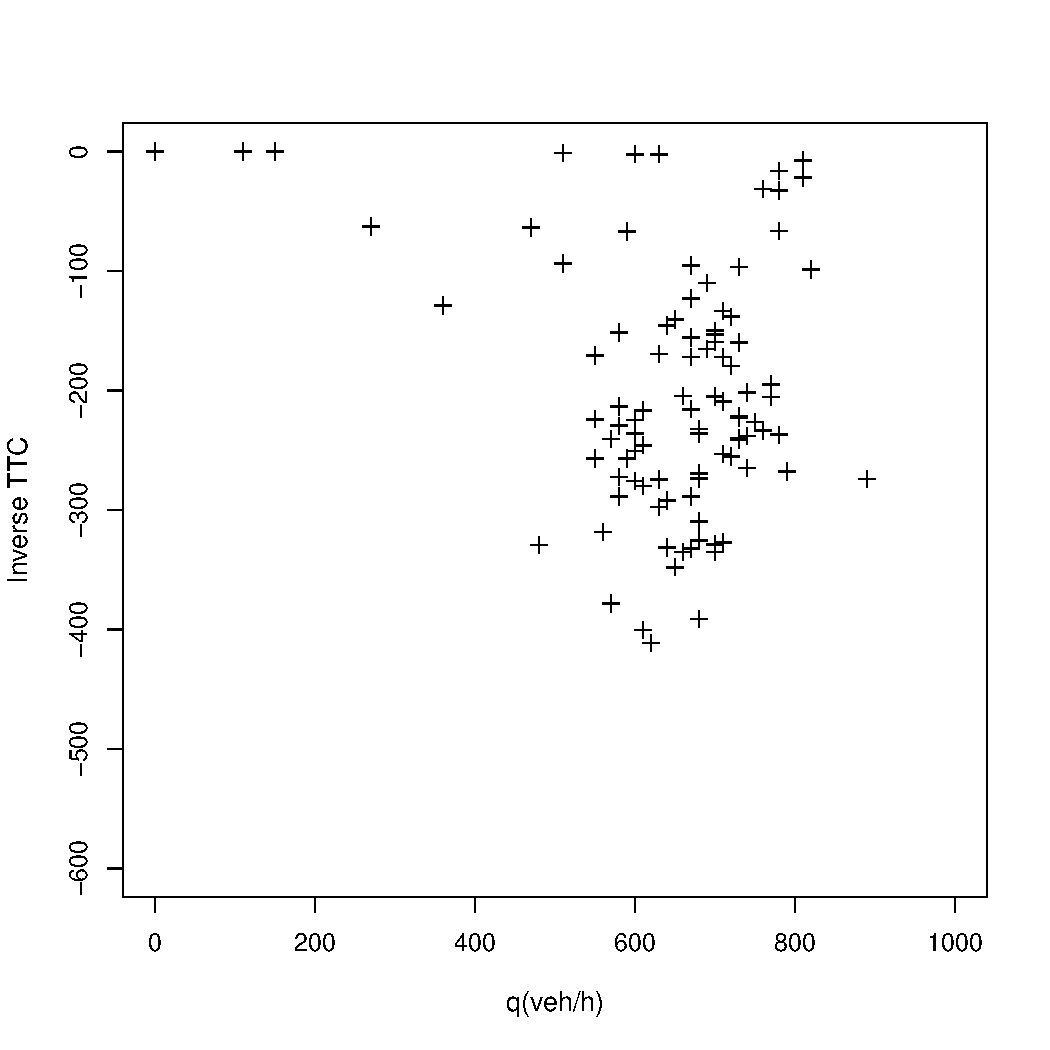
\includegraphics[width=0.33\linewidth]{factor1_ttc_per0}
}%
\subfloat[][]{%
\label{factor1_ttc_per25}%
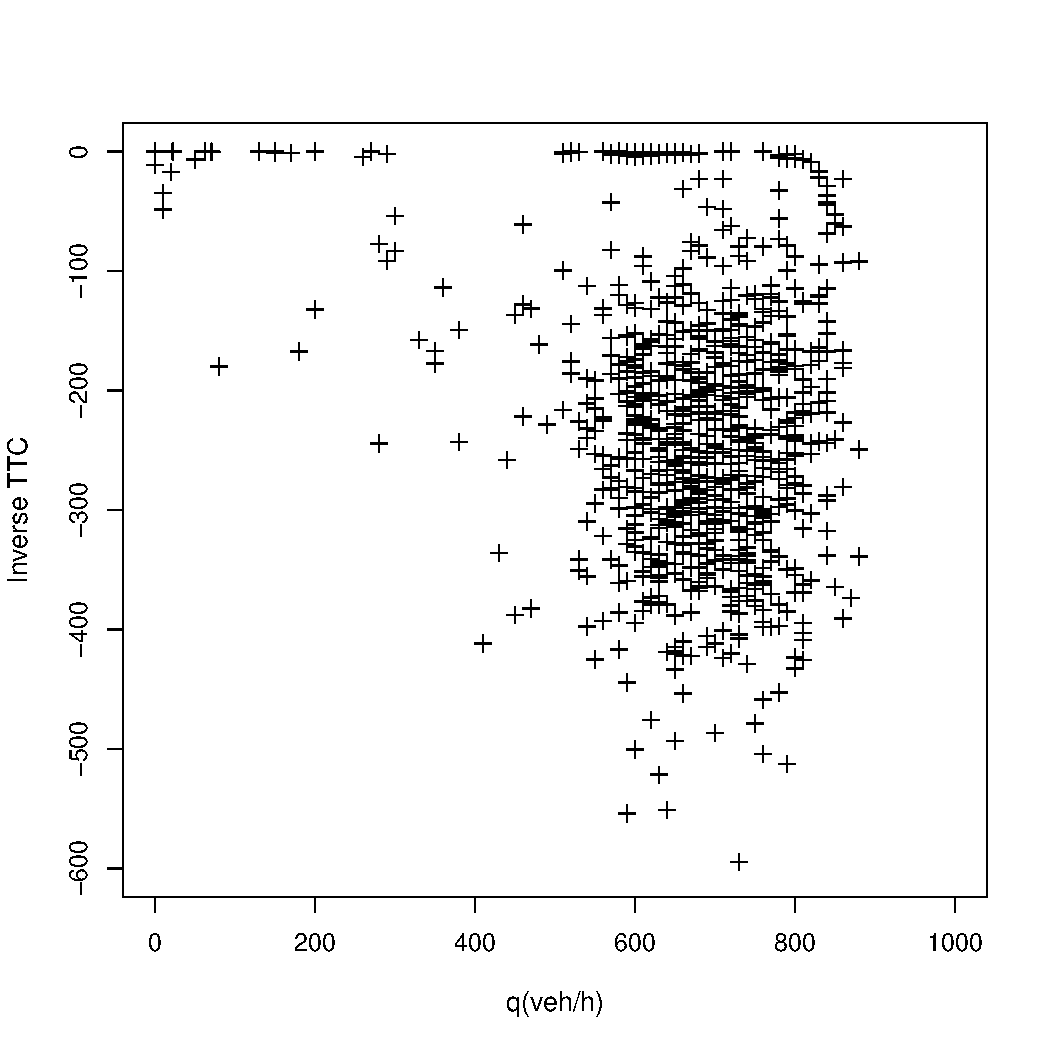
\includegraphics[width=0.33\linewidth]{factor1_ttc_per25}}
\subfloat[][]{%
\label{factor1_ttc_per50}%
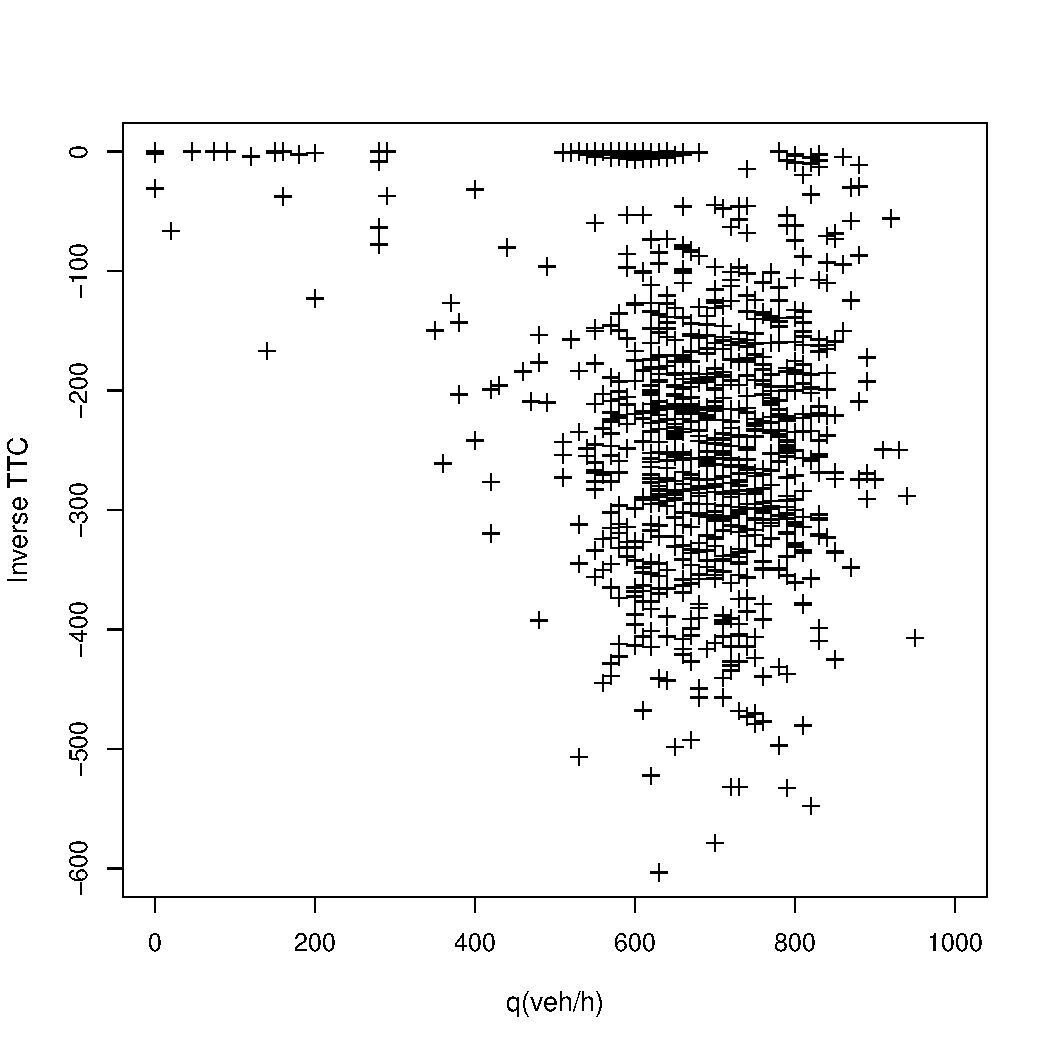
\includegraphics[width=0.33\linewidth]{factor1_ttc_per50}}\\%
\subfloat[][]{%
\label{factor1_ttc_per75}%
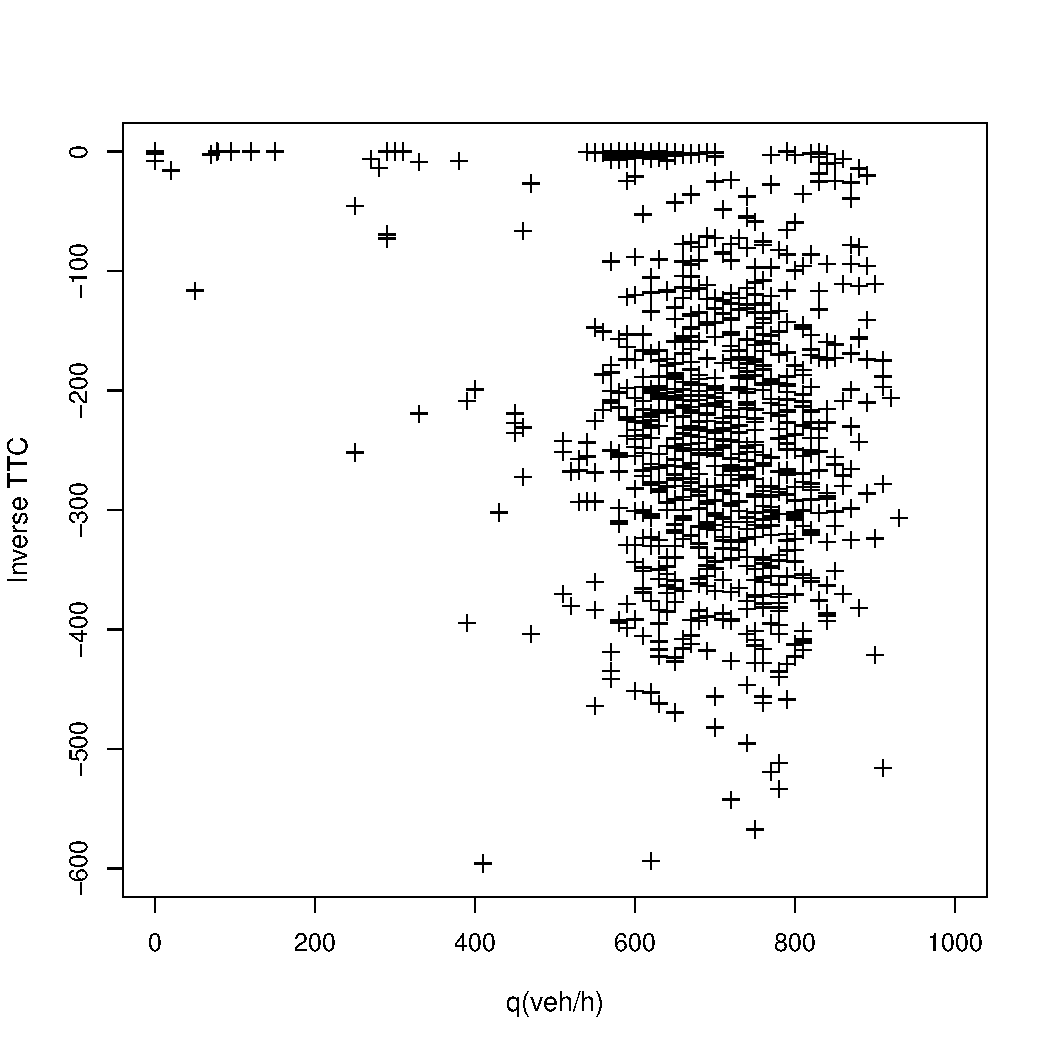
\includegraphics[width=0.33\linewidth]{factor1_ttc_per75}}%
\subfloat[][]{%
\label{factor1_ttc_per100}%
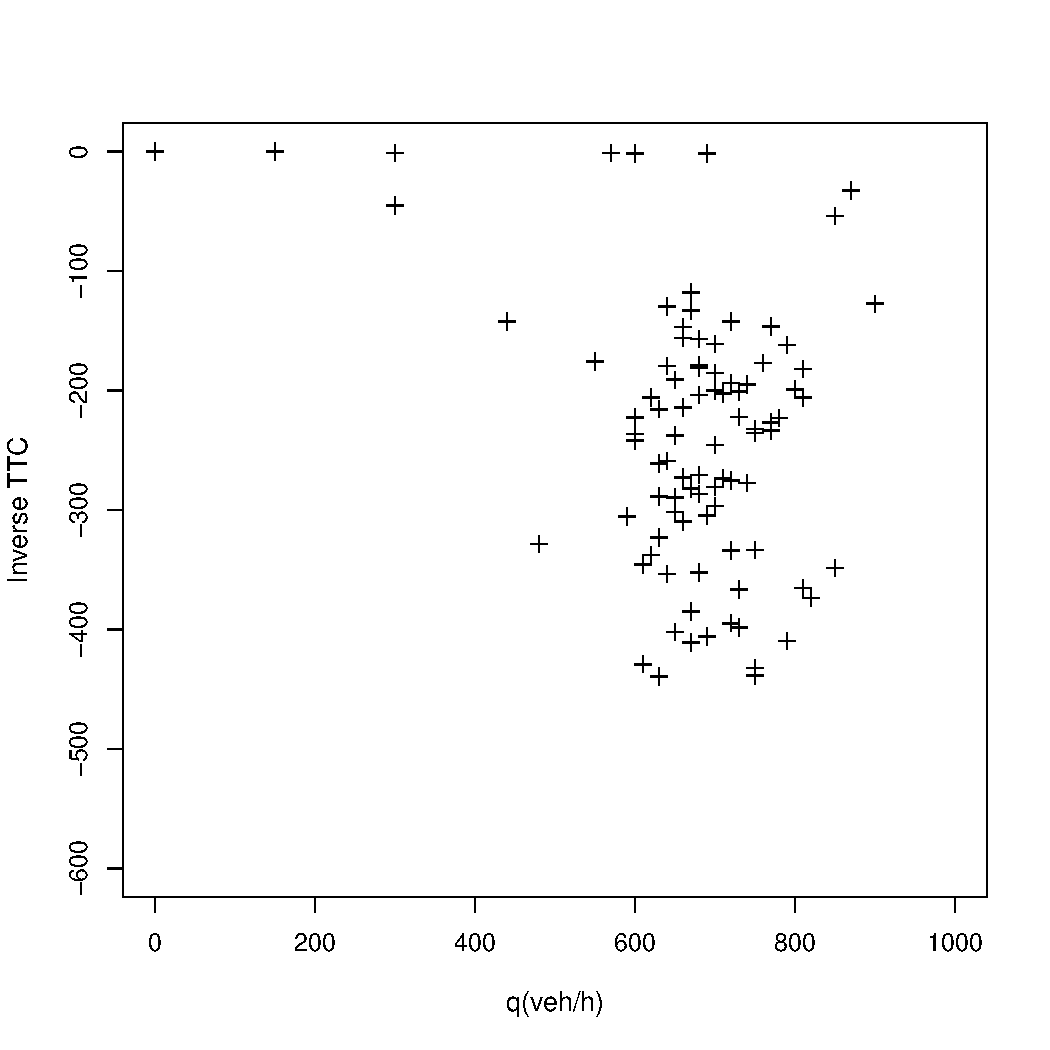
\includegraphics[width=0.33\linewidth]{factor1_ttc_per100}}
\caption[A set of four sub-floats.]{期望速度影响下流量与TTC倒数关系图
\subref{factor1_ttc_per0}
\subref{factor1_ttc_per25} 
\subref{factor1_ttc_per50}
\subref{factor1_ttc_per75}
\subref{factor1_ttc_per100}分别表示\autoref{speed-factor}中的B型驾驶人的百分比分别为0\%,25\%,50\%,75\%,100\%,其中流量为6个检测器平均值,TTC倒数为1分钟累计值}%
\label{factor1_ttc}%
\end{figure}

\begin{figure}[!htb]
\begin{center}
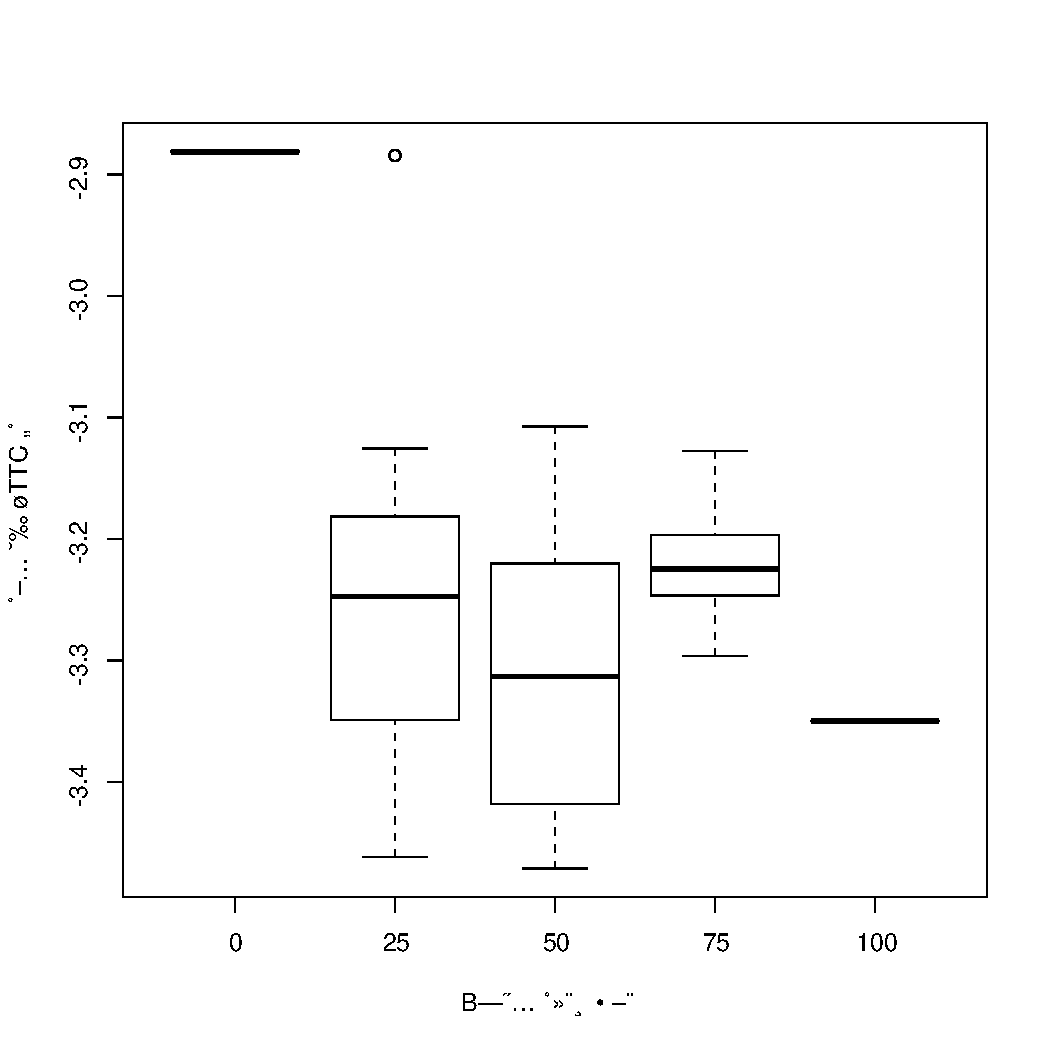
\includegraphics[width=0.7\linewidth]{factor1_box_avttc}
\caption{期望速度影响下时间平均TTC倒数箱图}
\label{factor1_box_avttc}
\end{center}
\end{figure}

\subsection{最大减速度影响因素}

最大减速度从\autoref{factor2_ttc}流量与TTC倒数关系图看,TTC倒数的和值的绝对值最大主要出现在流量600左右,从图上看对其分布没有显著影响。由\autoref{factor2_box_avttc}可以看出,期望车速对,时间平均TTC倒数(或者说TTC倒数的时间产生密度)的绝对值呈现先减少后增加的趋势,随着期望车速较高的B型驾驶人更多的混入,时间平均TTC倒数的绝对值呈现先减小后增加的趋势。这似乎说明存在一个最佳的B型驾驶人混入比例使得TTC倒数的实践产生密度绝对值最小。
\begin{figure}[!htb]%
\centering
\subfloat[][]{
\label{factor2_ttc_per0}%
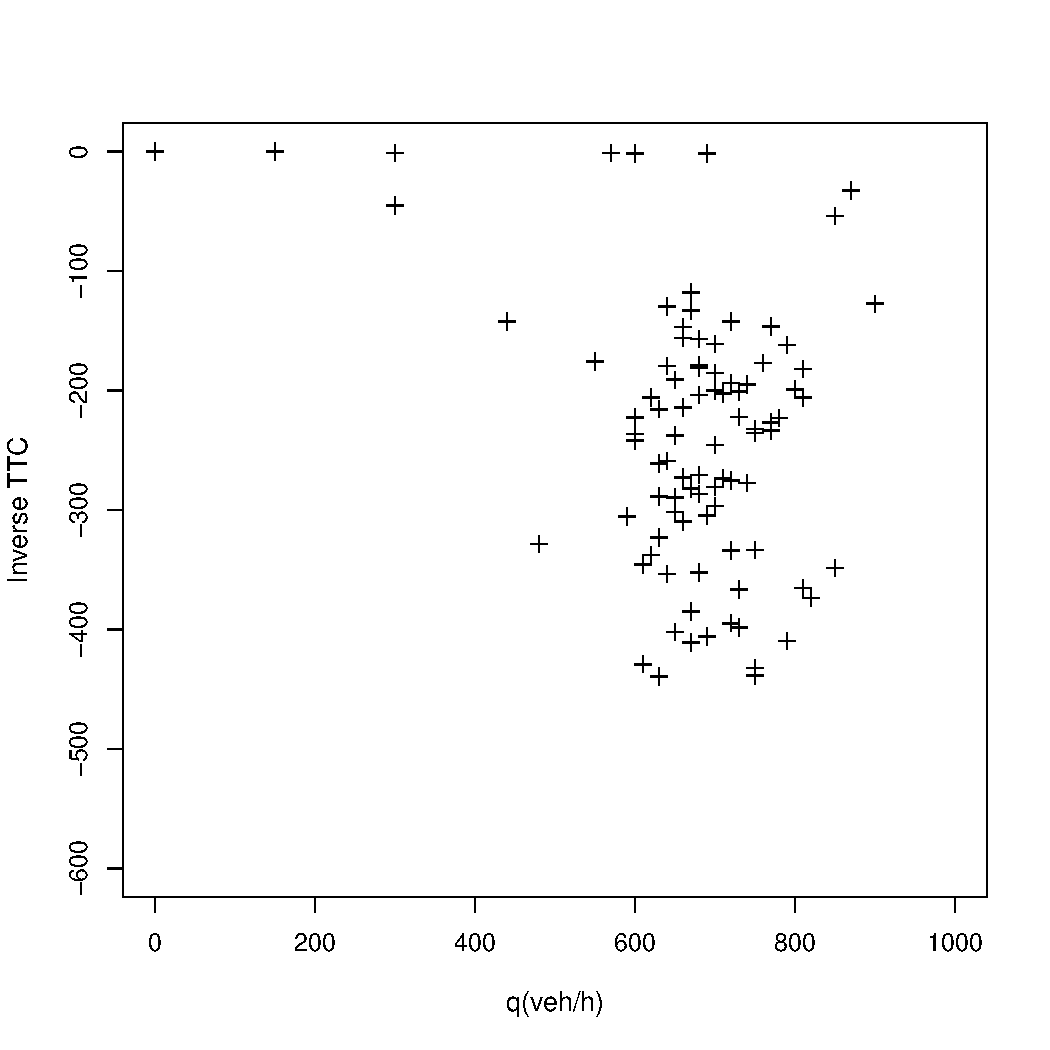
\includegraphics[width=0.33\linewidth]{factor2_ttc_per0}
}%
\subfloat[][]{%
\label{factor2_ttc_per25}%
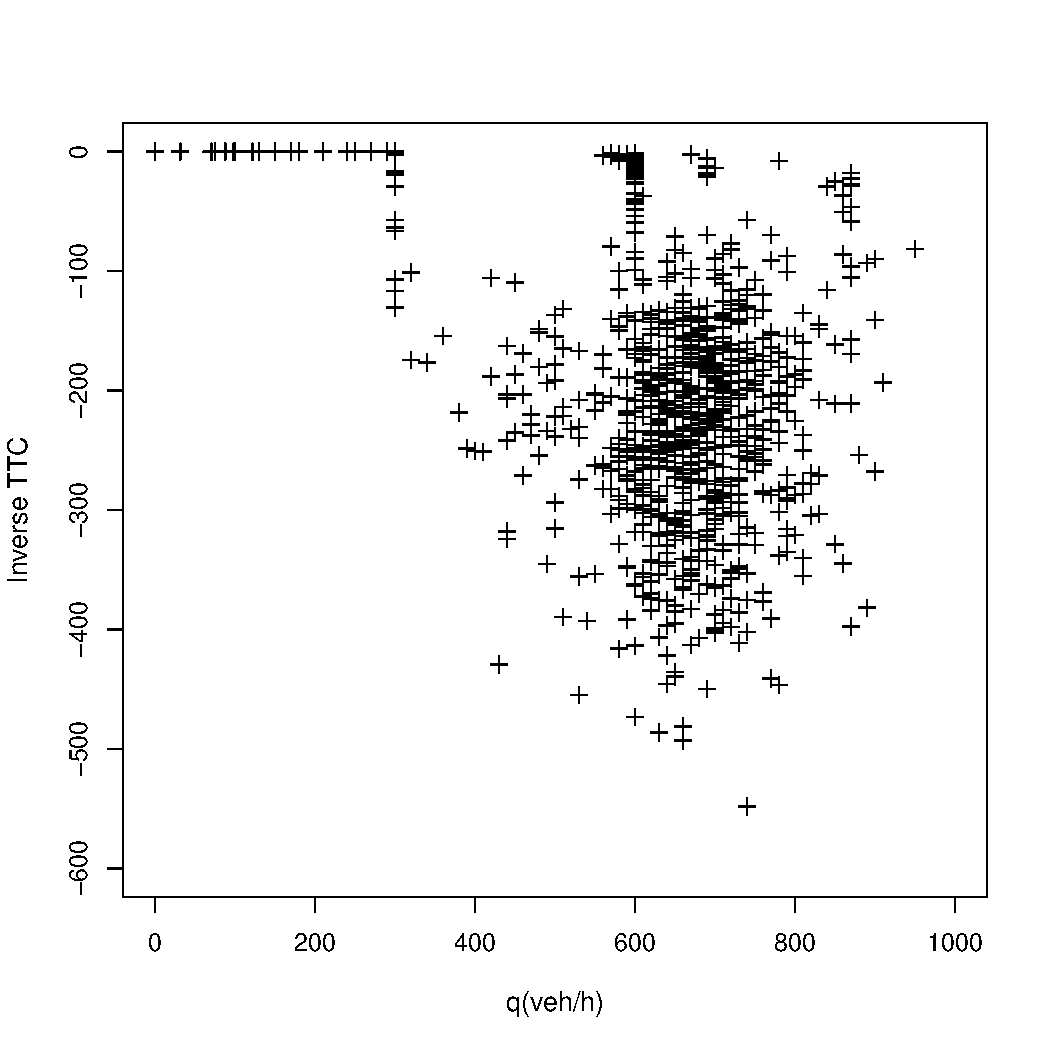
\includegraphics[width=0.33\linewidth]{factor2_ttc_per25}}
\subfloat[][]{%
\label{factor2_ttc_per50}%
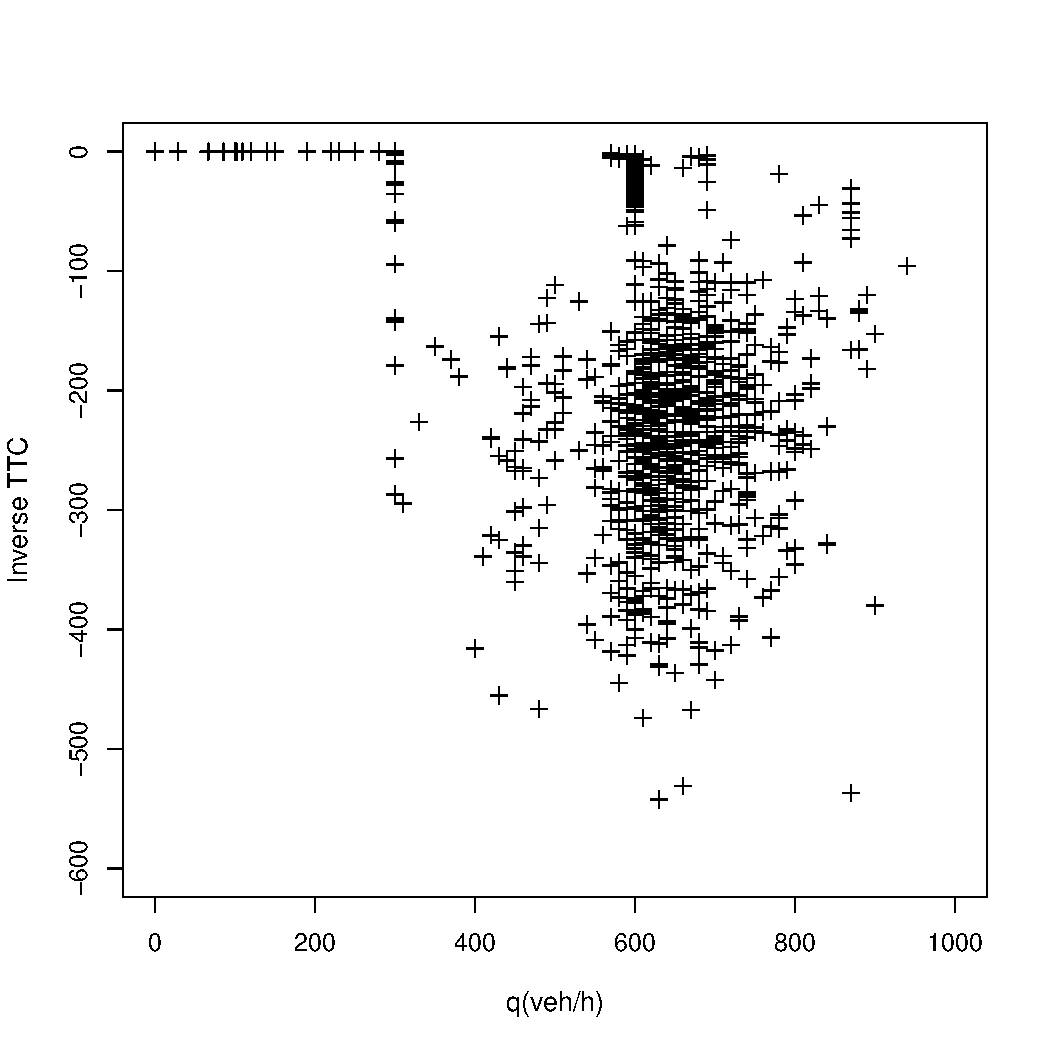
\includegraphics[width=0.33\linewidth]{factor2_ttc_per50}}\\%
\subfloat[][]{%
\label{factor2_ttc_per75}%
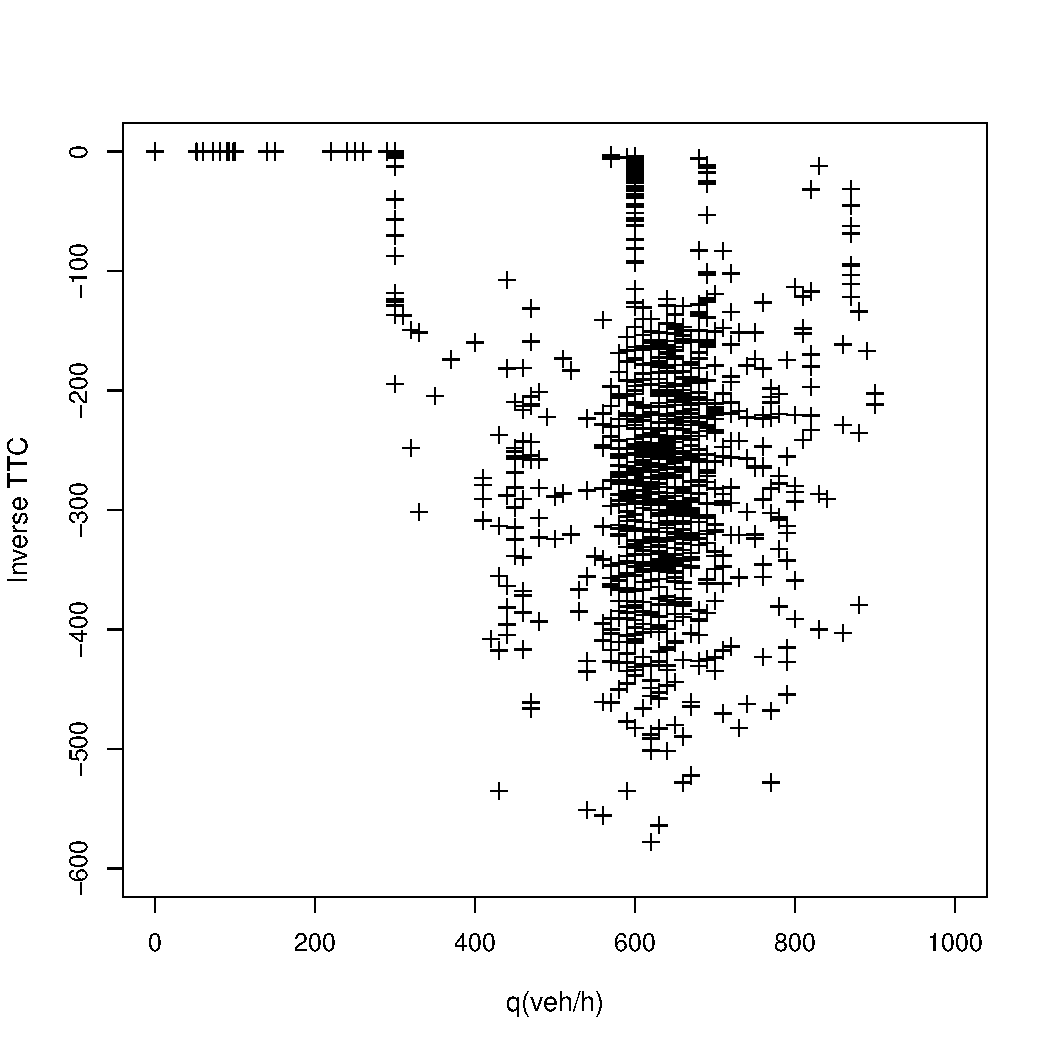
\includegraphics[width=0.33\linewidth]{factor2_ttc_per75}}%
\subfloat[][]{%
\label{factor2_ttc_per100}%
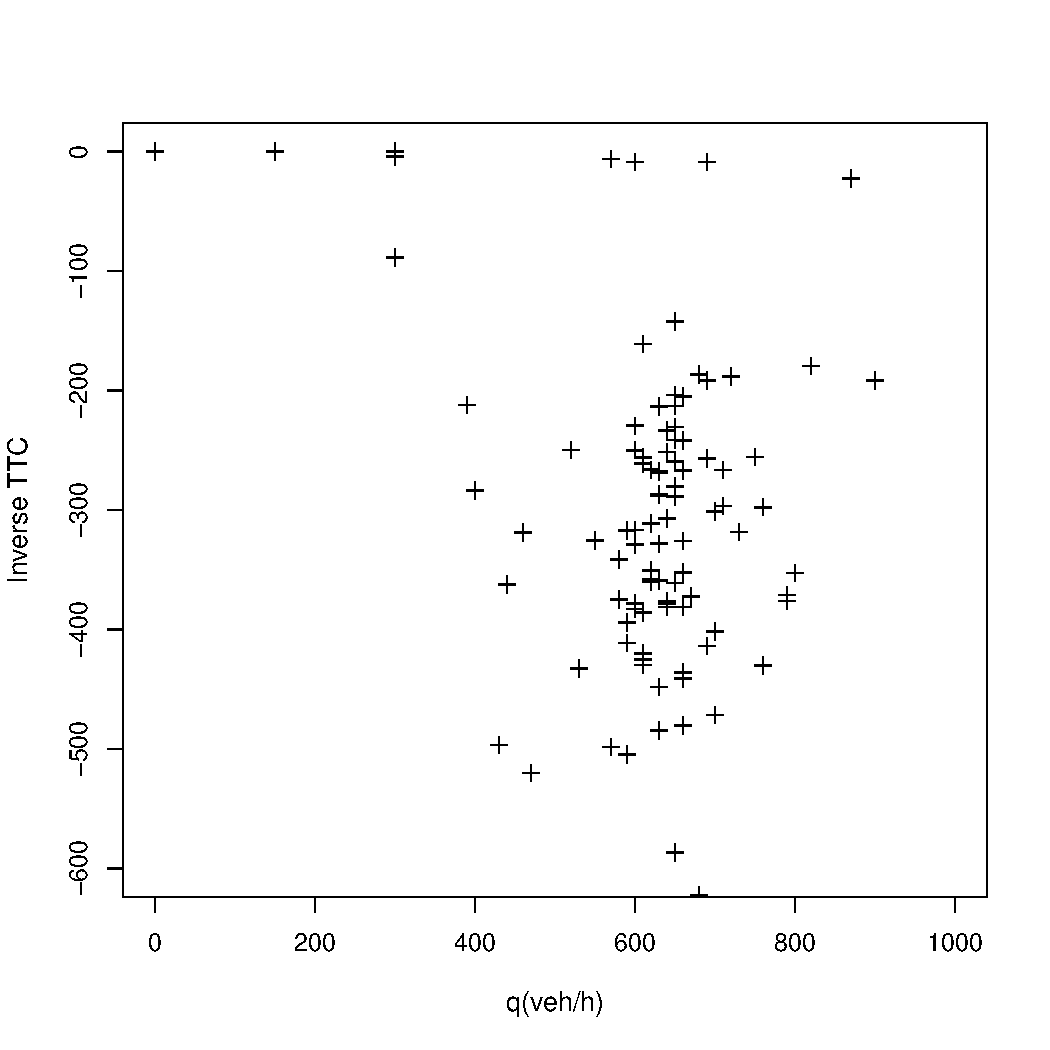
\includegraphics[width=0.33\linewidth]{factor2_ttc_per100}}
\caption[A set of four sub-floats.]{最大减速度影响下流量与TTC倒数关系图
\subref{factor2_ttc_per0}
\subref{factor2_ttc_per25} 
\subref{factor2_ttc_per50}
\subref{factor2_ttc_per75}
\subref{factor2_ttc_per100}分别表示\autoref{decel-factor}中的B型驾驶人的百分比分别为0\%,25\%,50\%,75\%,100\%,其中流量为6个检测器平均值,TTC倒数为1分钟累计值}%
\label{factor2_ttc}%
\end{figure}

\begin{figure}[!htb]
\begin{center}
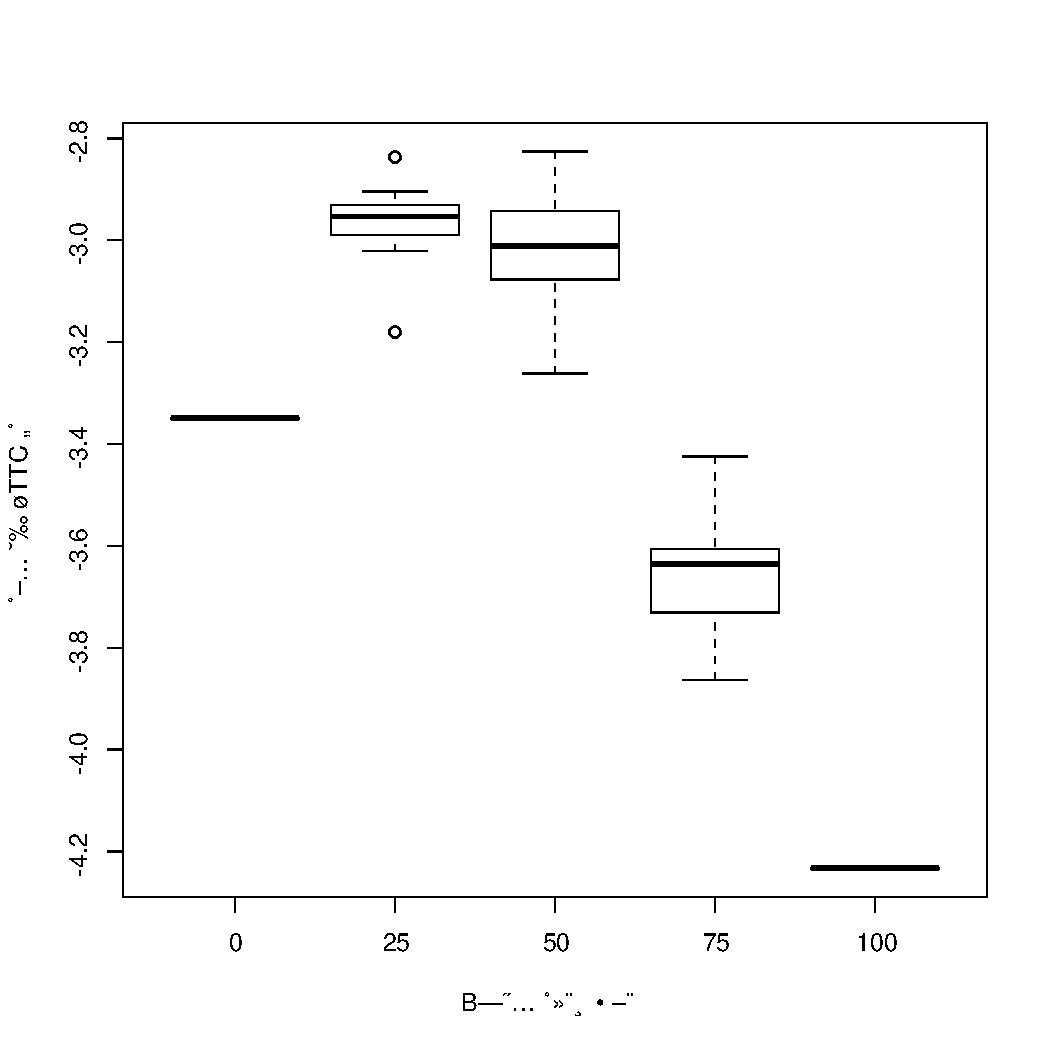
\includegraphics[width=0.7\linewidth]{factor2_box_avttc}
\caption{最大减速度影响下时间平均TTC倒数箱图}
\label{factor2_box_avttc}
\end{center}
\end{figure}

\subsection{混合影响因素}

混合作用影响下的结果与最大减速影响的结果相似,这再一次表明最大减速度是影响交通流的主要因素。
\begin{figure}[!htb]%
\centering
\subfloat[][]{
\label{combined_ttc_per0}%
\includegraphics[width=0.33\linewidth]{combined_ttc_per0}
}%
\subfloat[][]{%
\label{combined_ttc_per25}%
\includegraphics[width=0.33\linewidth]{combined_ttc_per25}}
\subfloat[][]{%
\label{combined_ttc_per50}%
\includegraphics[width=0.33\linewidth]{combined_ttc_per50}}\\%
\subfloat[][]{%
\label{combined_ttc_per75}%
\includegraphics[width=0.33\linewidth]{combined_ttc_per75}}%
\subfloat[][]{%
\label{combined_ttc_per100}%
\includegraphics[width=0.33\linewidth]{combined_ttc_per100}}
\caption[A set of four sub-floats.]{混合作用影响下流量与TTC倒数关系图
\subref{combined_ttc_per0}
\subref{combined_ttc_per25} 
\subref{combined_ttc_per50}
\subref{combined_ttc_per75}
\subref{combined_ttc_per100}分别表示\autoref{combined-factor}中的B型驾驶人的百分比分别为0\%,25\%,50\%,75\%,100\%,其中流量为6个检测器平均值,TTC倒数为1分钟累计值}%
\label{combined_ttc}%
\end{figure}

\begin{figure}[!htb]
\begin{center}
\includegraphics[width=0.7\linewidth]{combined_box_avttc}
\caption{混合作用影响下时间平均TTC倒数箱图}
\label{combined_box_avttc}
\end{center}
\end{figure}

\section{本章小结}



%\begin{figure}[htb] 
%  \begin{minipage}[b]{0.3\linewidth} 
%
%  \end{minipage}% 
%  \begin{minipage}[b]{0.3\linewidth} 
%
%  \end{minipage} 
%  \begin{minipage}[b]{0.3\linewidth} 
%
%  \end{minipage} 
%\end{figure}



%\begin{figure}[htb] 
%  \begin{minipage}[b]{0.33\linewidth} 
%\begin{center}
%\includegraphics[width=\linewidth]{factor1_vq_per0}
%\end{center}
%\caption{模拟场景图}
%\label{factor1_vq_per0}
%  \end{minipage}% 
%  \begin{minipage}[b]{0.33\linewidth} 
%\begin{center}
%\includegraphics[width=\linewidth]{factor1_vq_per25}
%\end{center}
%\caption{模拟场景图}
%\label{factor1_vq_per25}
%  \end{minipage} 
%  \begin{minipage}[b]{0.33\linewidth} 
%\begin{center}
%\includegraphics[width=\linewidth]{factor1_vq_per50}
%\end{center}
%\caption{模拟场景图}
%\label{factor1_vq_per50}
%  \end{minipage}
%\hspace*{0.17\linewidth}
%  \begin{minipage}[b]{0.33\linewidth} 
%\begin{center}
%\includegraphics[width=\linewidth]{factor1_vq_per75}
%\end{center}
%\caption{模拟场景图}
%\label{factor1_vq_per75}
%  \end{minipage}
%  \begin{minipage}[b]{0.33\linewidth} 
%\begin{center}
%\includegraphics[width=\linewidth]{factor1_vq_per100}
%\end{center}
%\caption{模拟场景图}
%\label{factor1_vq_per100}
%  \end{minipage}
%\end{figure}